%% Plantilla para informes de trabajos de grado del Programa de Ingeniería
%% Electrónica de la Universidad de Nariño. Este docuemento es una
%% modificación de la plantilla IEEE cuya información legal y de licencia
%% se encuentra a continuación


%% bare_jrnl.tex
%% V1.4b
%% 2015/08/26
%% by Michael Shell
%% see http://www.michaelshell.org/
%% for current contact information.
%%
%% This is a skeleton file demonstrating the use of IEEEtran.cls
%% (requires IEEEtran.cls version 1.8b or later) with an IEEE
%% journal paper.
%%
%% Support sites:
%% http://www.michaelshell.org/tex/ieeetran/
%% http://www.ctan.org/pkg/ieeetran
%% and
%% http://www.ieee.org/

%%*************************************************************************
%% Legal Notice:
%% This code is offered as-is without any warranty either expressed or
%% implied; without even the implied warranty of MERCHANTABILITY or
%% FITNESS FOR A PARTICULAR PURPOSE! 
%% User assumes all risk.
%% In no event shall the IEEE or any contributor to this code be liable for
%% any damages or losses, including, but not limited to, incidental,
%% consequential, or any other damages, resulting from the use or misuse
%% of any information contained here.
%%
%% All comments are the opinions of their respective authors and are not
%% necessarily endorsed by the IEEE.
%%
%% This work is distributed under the LaTeX Project Public License (LPPL)
%% ( http://www.latex-project.org/ ) version 1.3, and may be freely used,
%% distributed and modified. A copy of the LPPL, version 1.3, is included
%% in the base LaTeX documentation of all distributions of LaTeX released
%% 2003/12/01 or later.
%% Retain all contribution notices and credits.
%% ** Modified files should be clearly indicated as such, including  **
%% ** renaming them and changing author support contact information. **
%%*************************************************************************


% *** Authors should verify (and, if needed, correct) their LaTeX system  ***
% *** with the testflow diagnostic prior to trusting their LaTeX platform ***
% *** with production work. The IEEE's font choices and paper sizes can   ***
% *** trigger bugs that do not appear when using other class files.       ***                          ***
% The testflow support page is at:
% http://www.michaelshell.org/tex/testflow/



\documentclass[journal]{IEEEtran}	% Requiere la instalación de la clase IEEEtran


%% Algunos paquetes útiles %%

\usepackage{amsmath}		% Para símbolos matemáticos
\usepackage{amssymb}		% Para símbolos matemáticos
\usepackage{amsthm}			% Para símbolos matemáticos
\usepackage{mathtools}		% Para símbolos matemáticos
\usepackage{mathdots}		% Para símbolos matemáticos
\usepackage{epstopdf}		% Para figuras
%\usepackage[spanish,es-tabla,es-nodecimaldot]{babel} % Para redacción en español
\usepackage[T1]{fontenc} 							 % Para redacción en español
\usepackage[utf8]{inputenc}							 % Para redacción en español
\usepackage[hidelinks]{hyperref}
\usepackage{float}
\usepackage{graphicx}

% *** No ajuste los márgenes, columnas ni tamaños de las fuentes ***

% ** Librerias externas para graficos
\usepackage{tikz}
\usepackage{listings}
\usepackage{xcolor}
\usepackage{dirtree}

\usetikzlibrary{shadows.blur}
\usetikzlibrary{arrows,automata}

\tikzset{% 
	gateway/.style={circle, draw=none, fill=IntelBlue,
		text centered, anchor=north, text=white,
		blur shadow={shadow blur steps=10,shadow blur extra rounding=1.3pt}},
	server/.style={circle, draw=none, fill=BlueViolet,
		text centered, anchor=north, text=white,
		blur shadow={shadow blur steps=5,shadow blur extra rounding=1.3pt}},
	gva/.style={circle, draw=none, fill=RawSienna,
		text centered, anchor=north, text=white,
		blur shadow={shadow blur steps=5,shadow blur extra rounding=1.3pt}},
	leaf/.style={circle, draw=none, fill=Green,
		text centered, anchor=north, text=white,
		blur shadow={shadow blur steps=5,shadow blur extra rounding=1.3pt}},
}

% Definicion variables globales
\xglobal\definecolor{IntelBlue}{RGB}{0,113,197}
\xglobal\definecolor{RawSienna}{RGB}{197,113,50}
\xglobal\definecolor{BlueViolet}{RGB}{100,0,240}
\xglobal\definecolor{Green}{RGB}{0,150,100}

%New colors defined below
\definecolor{codegreen}{rgb}{0,0.6,0}
\definecolor{codegray}{rgb}{0.5,0.5,0.5}
\definecolor{codepurple}{rgb}{0.58,0,0.82}
\definecolor{backcolour}{rgb}{0.95,0.95,0.92}

%Code listing style named "mystyle"
\lstdefinestyle{mystyle}{
  backgroundcolor=\color{backcolour},   commentstyle=\color{codegreen},
  keywordstyle=\color{magenta},
  morekeywords={Title, Feature, Scenario, Given, And, When, Then}, 
  keywordstyle=\bfseries\color{purple!40!black},
  numberstyle=\tiny\color{codegray},
  stringstyle=\color{codepurple},
  basicstyle=\ttfamily\footnotesize,
  breakatwhitespace=false,         
  breaklines=true,                 
  captionpos=b,                    
  keepspaces=true,                 
  numbers=left,                    
  numbersep=5pt,                  
  showspaces=false,                
  showstringspaces=false,
  showtabs=false,                  
  tabsize=2
}

%"mystyle" code listing set
\lstset{style=mystyle}

\lstdefinestyle{okstyle}{
    language=java,
    moredelim=**[is][\color{green!60!black}]{&}{&},
    moredelim=**[is][\color{red!60!black}]{[}{]},
    moredelim=**[is][\color{green}]{@}{@},
    moredelim=**[is][\color{red}]{<}{>},
    moredelim=**[is][\color{gray}]{*}{*},
    morekeywords={Title, Feature, Scenario}, 
    keywordstyle=\color{white}\bfseries,
    basicstyle=\ttfamily\footnotesize\color{white},
    backgroundcolor=\color{black},
    breaklines=true,
    columns=fullflexible,
}

\lstdefinestyle{scenarioStyle}{
    moredelim=**[is][\color{green!65!blue}]{&}{&},
    moredelim=**[is][\color{orange!80!white}]{<}{>},
    moredelim=**[is][\color{white}]{-}{-},
    morekeywords={Title, Feature, Scenario, Given, When, Then, And}, 
    keywordstyle=\color{cyan!60!black}\bfseries,
    basicstyle=\ttfamily\footnotesize\color{white},
    backgroundcolor=\color{white!15!black},
    breaklines=true,
    columns=fullflexible,
}

\renewcommand{\lstlistingname}{Algorithm}


%% Inicio del documento
\begin{document}

% Título con las primeras letras en mayúsculas excepto palabras cortas como 'de'
% o preposiciones.
\title{Design and Implementation of a System to Manage the Automatic Behavioral Testing of an IoT Environment for the TaIO Systems Company}

% Nombres de los autores. No edite el pie de página que empieza con \thanks
\author{Juan David Velasquez Rosero \\Advisor: PhD. Wilson O. Achicanoy-Martínez.\\Company Advisor: PhD. Juan Pablo Ruiz Rosero.\\Departament of Electronics Engineering\\
Universidad de Nariño % <-this % stops a space
\thanks{Thesis dissertation presented as a requirement to get the title of Electronics Engineer at Universidad de Nariño, Pasto, Colombia. June 7, 2021.}
\thanks{Juan David Velasquez Rosero (2121601297). Student, Electronics Engineering Program, email: \href{juand.vr28@gmail.com}{juand.vr28@gmail.com}}
\thanks{PhD. Wilson O. Achicanoy M., Assistant Professor, Department of Electronics Engineering, email:~\href{wilachic@udenar.edu.co}{wilachic@udenar.edu.co}}
\thanks{PhD. Juan Pablo Ruiz Rosero, Director, TaIO Systems, email:~\href{juan.ruiz@taiosystems.com}{juan.ruiz@taiosystems.com}}}




% Encabezados de páginas pares e impares. No modificar
\markboth{Programa de Ingeniería Electrónica, Universidad de Nariño}%
{Programa de Ingeniería Electrónica, Universidad de Nariño}


% Crea el área del título
\maketitle


% Resumen
\begin{abstract}


Software development techniques are a fundamental part of Software Engineering Theory. Suitable planning and validation of a computer system's characteristics contribute positively to its maintenance, scalability, and error correction. Nowadays, a widely used technique is Behavior-Based Development, which has advantages over other methods such as TDD (Test Driven Development). It uses natural language to describe system's scenarios to be evaluated in tests, and when failures occur, it allows easy communication between the different levels that make up a company. The current strong demand for this technique is evident in software development for a variety of purposes, but its implementation in the Internet of Things (IoT) systems has not been sufficiently documented.

The purpose of this thesis aimed to design and implement a system to manage the automatic behavior tests of an IoT environment, in order to detect errors and verify compliance with the system's requirements and functionalities. In addition, it allows agile and efficient information handling on failures and communication between developers, testers, and other participants in the business environment. To achieve this objective, the main characteristics that describe the operation of the IoT system and their respective programming languages were studied, and an optimal strategy was implemented the build a test tool taking into account the current conditions on hardware and software from which it is made. The validation of the design and implementation of the application was made for a case study supervised by the TaIO Systems staff.


\end{abstract}


% No es necesario usar palabras clave. El siguiente código sirve para incluirlas si lo considera necesario
%\begin{IEEEkeywords}
%IEEE, IEEEtran, journal, \LaTeX, paper, template.
%\end{IEEEkeywords}


\section{Introduction}


% La primera palabra de la introducción debe usar el formato tradicional dado por \IEEEPARstart
%La introducción debe contener la definición del problema, el estado del arte (o trabajos relacionados) y las contribuciones realizadas en el trabajo de grado.


\subsection{Problem definition}


\IEEEPARstart{I}n recent decades, technological advances have been presented with a great impact on different aspects of our daily lives. The growth of communication networks around the world and access to the Internet have produced significant changes in the way we communicate with each other and the way we connect or relate to the “things” that surround us. The latter is known as the Internet of Things (IoT). The IoT is an ecosystem that is constantly growing and integrates hardware, software, computing devices, physical objects, and animals or people, through a network that allows them to interact, communicate, and collect and exchange data. The IoT has become a technological tool with the potential to solve problems in different areas such as medicine \cite{farahani2018towards,aktas2018iot,chen2015low}, security \cite{mao2018application}, entertainment \cite{kumar2019iot}, vehicle tracking and transport vehicles \cite{lee2014design,jisha2017iot}, transportation and parcel industry \cite{caballero2013iot,li2017iot}, and agriculture \cite{davcev2018iot,elijah2018overview}. Currently, it strengthens other technologies by collecting large amounts of information for use in training of Machine Learning algorithms and Big Data applications \cite{syafrudin2018performance,cai2016iot,luo2019development}.

These digital ecosystems involve large amounts of connected electronic devices, and their implementation requires different development platforms, programming languages, and experts in the different phases of the development process. To be released into production, correct operation of IoT systems and their electronic and computer parts, such as servers, microprocessors, microcontrollers, power supplies, sensor networks, communication protocols, encryption mechanisms, etc., each with different characteristics, must be described, understood, and validated. And it should be noted that the issue of software quality has been systematically discussed since the early 1980s with the concept of software engineering. From there, various methods and techniques have emerged and aimed to ensure the quality of computer systems. More recently, Behavior Driven Development (BDD) has gained greater acceptance by offering a mechanism to ensure that the software performs as expected, getting it to be adopted by different agile development methods \cite{nascimento2020behavior}.

Finally, it is important to mention that the time of development and correction of faults is an issue of vital importance for companies. The absence or poor execution of tools that guide the development and validation of an electronic and computer system generates delays in delivery times, high maintenance costs, long periods of fault correction, and maximization of project risks. Moreover, the omission of methods of software development and validation techniques can generate communication problems into the development team, when transferring information about failures and including a disarticulation between the requirements and needs of the end user and its functionalities. On the other hand, the presence of the aforementioned shortcomings can lead to a lack of trust between developers and testers, due to a decrease in their ability to predict and understand the structure of their work. This is the reason why the BDD concept acquires great importance in this type of application, being an appropriate way to verify the operation of the system, understood as a set of scenarios that describe the different characteristics that make up its multiplatform structure \cite{nascimento2020behavior,soeken2012assisted,north2010introducing}.


\subsection{State of the art}


The development of computer systems using the behavior-based method has been analyzed as a starting point for the approach proposed in this project. The current state of the art is the result of an investigation carried out on the most significant projects that have been found in engineering databases.

In Brazil, Hugo Lopes Tavares et al. present a set of tools for the implementation, specification, and testing of software following BDD practices coded in the language Python \cite{tavares2010tool}. The authors conclude that the use of these test tools highlights the specification and validation of the expected behavior of the software, reducing the error rate and improving the documentation. Thus, it is possible to produce code with far fewer defects at the behavioral and unit level, as well as better meet development expectations.

In \cite{solis2011study}, Carlos Solís and Xiaofeng Wang developed a study of the characteristics of BDD, in which they describe its main characteristics identified through an analysis of the corresponding literature and present the commonly used tools to implement this method. They providing a basis for understanding BDD as well as for expanding existing BDD tool sets or developing new ones.

Recently, in 2019, Myint Myint Moe publishes in the International Journal of Trends in Scientific Research and Development (IJTSRD) a comparative study between three software development techniques: TDD (Test Driven Development), BDD (Behavior Driven Development), and ATDD (Acceptance Test-Driven Development), in which he describes the main advantages and disadvantages of each of the methods \cite{moe2019comparative}. The authors mention that BDD has evolved from TDD as a format to eliminate the deficiencies of TDD, highlighting better communication between developers, testers and users. They also highlight a much shorter learning curve as a consequence of the use of natural language. But this method also has some disadvantages when the requirements and functionalities of the system are not specified properly. Furthermore, the authors assure that to work with BDD, prior knowledge of other testing methodologies such as TDD is required.

In the same year, Mohammad Alhaj, Gilbert Arbez and Liam Peyton published a study on the integration of behavioral development with hardware and software co-design, applied to a renewable energy project in collaboration with a private company in Canada. The goal is to build a system of autonomous load management of self-forming renewable energy nano-grids \cite{alhajapproach}.

Finally, in 2021, Behave provides an open source repository oriented to the implementation of the agile BDD technique over Python language \cite{behave2021github}. Both the documentation and the developer community forums found in this source were the basis for coding the behavioral testing tool of this work.


\subsection{Work contributions}

In this project, an automatic behavioral testing system based on BDD methodology is designed and implemented for an IoT environment. One hundred real testing scenarios are probed by facing the system to different conditions like those based on the number of sensor nodes, percentage of lost packets, and disconnection periods, among others things. The performance of the automatic behavioral testing system is measured by taking into account the speed factor against execution in a real environment, capacity for agile debugging, correction of bugs, and development of new functionalities.

To achieve the above objective, a case study for the operation of an IoT environment is carried out by simulation. In this simulation, the system is capable of executing all the components of the IoT environment on a computer with Linux operating system. It simulates all the system's components and the different communication channels that connect them. In addition, a synchronization mechanism is developed for multiple processes running over different programming languages.



\section{TaIO Systems Company and IoT case study}


TaIO Systems is a company located in the city of Popayán (Colombia), which has a human team with extensive professional and academic knowledge for management of integrated systems, firmware development, mobile application development, and information and communications technology (ICT) projects. TaIO Systems has successfully supported Intel Corporation on various projects, as an independent consulting and development company, that specializes in providing services such as firmware, mobile systems, and prototypes for hardware peripherals based on common technologies such as Bluetooth 4.0/5.0, RFID, Zigbee, and LoRa.

In terms of hardware design, TaIO Systems has extensive experience designing devices under size and power constraints. In the case of mobile systems, they have developed applications on iOS and Android platforms for hybrid systems over smartphones, using different types of interconnection (Wi-Fi, NFC, Bluetooth, USB, etc.) and different types of sensors. Besides, the company develops prototypes using standard software engineering techniques and rigorous test plans. These prototypes are necessary for the validation of architectures and decision-making in information and communication technology (ICT) projects.

Currently, the company is developing a project in the context of logistics and asset management. The purpose of this project is to track packages that are delivered using different modes of transport. It is important to watch variables such as tilt, temperature, humidity, location, shock, and pressure (see Fig.~\ref{fig:logistic1}).

\begin{figure}[t!]
\centering
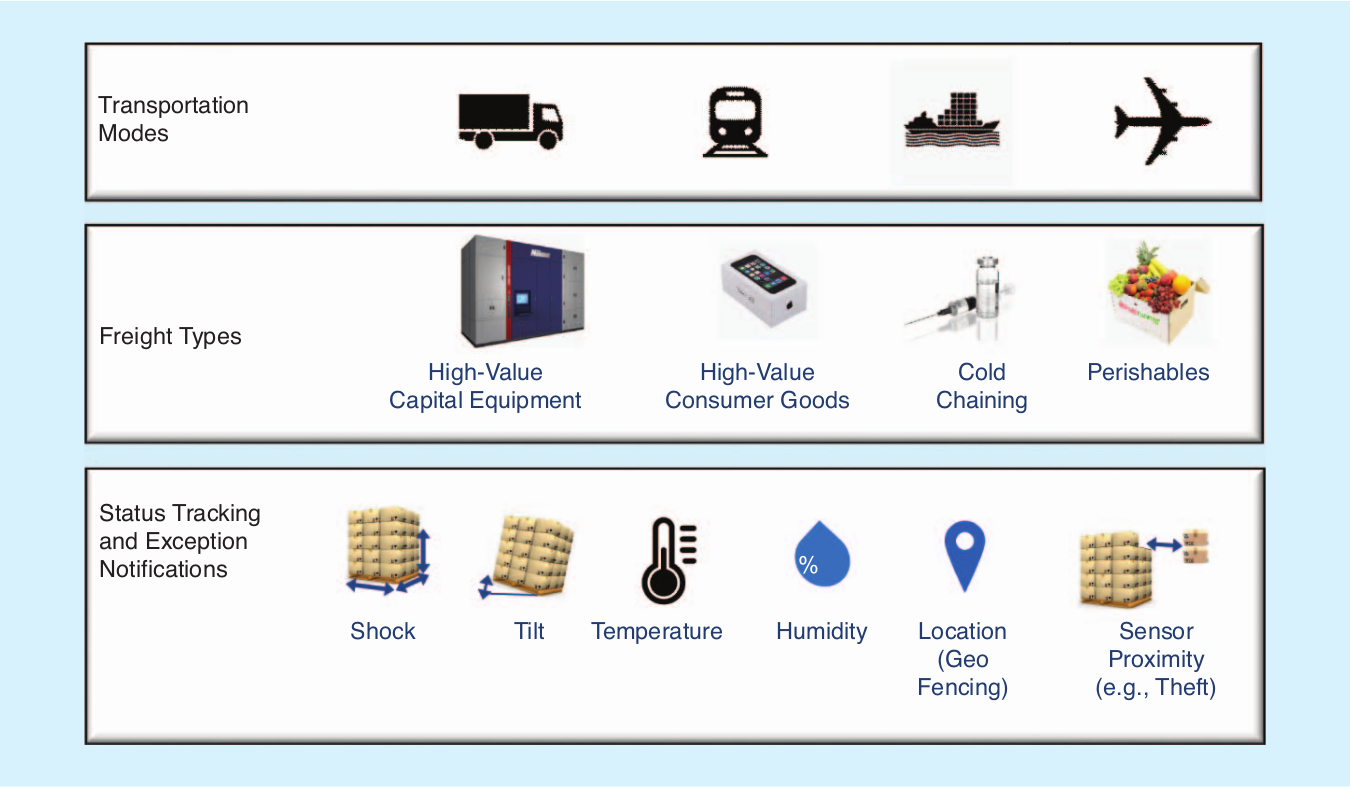
\includegraphics[width=1.0\columnwidth]{fig1.png}
\caption{Logistics and asset management across diverse transportation modes and freight types. Source: Adapted from \cite{williams2017weaving}}.
\label{fig:logistic1}
\end{figure}

In this project, the developed system fall within the Wireless Sensor Network and Internet of Things (WSN-IoT) category. The system includes: (i) a set of nodes called "Tags", that are attached to the packets or loads; (ii) one or more devices called "Unified Gateway Server", that act as a gateway between the 2.4 GHz LR-WPAN (Low-Rate Wireless Personal Area Network) and the data transmission to the cloud via Wi-Fi or the cellular network; and (iii) multiple cloud modules, which allow communication between  the devices, to monitor and to configure system's characteristics, and data visualization. Thus, it is achieved greater operational efficiency in the system \cite{williams2017weaving}.


\section{Description of the operation and components of the IoT environment}


As mentioned in the previous section, the main system components are the tags, the Unified Gateway Server device, and the cloud modules, which together are called Gateway Virtual Appliance (GVA). Below, these parts are described in detail.


\subsection{Structure of the IoT environment}


In this IoT environment, it is used a star network topology in which the nodes are identified as server and client, based on their operations. Fig. \ref{fig:topology} shows this topology. The client node is a physical device (tag) used for in situ data collection from environmental and device health sensors. The server (or coordinator) node can have the same hardware as a client, but acts as either a Personal Area Network coordinator (PAN coordinator) and aggregator of sensor data from its client nodes. The clients are equipped with sensors and must be provisioned to associate with an assigned server, which can be connected to an Internet-enabled GW for cloud services. Each device is battery operated with limited resources, and each server-clients network operates on a shared 15.4 wireless channel, using a synchronous time-division multiplexing (TDM) schedule guided by local timers and WSN packet payloads. These mechanisms are explained in more detail in section \ref{sub:tag_server}.

\begin{figure}[t!]
    \centering
    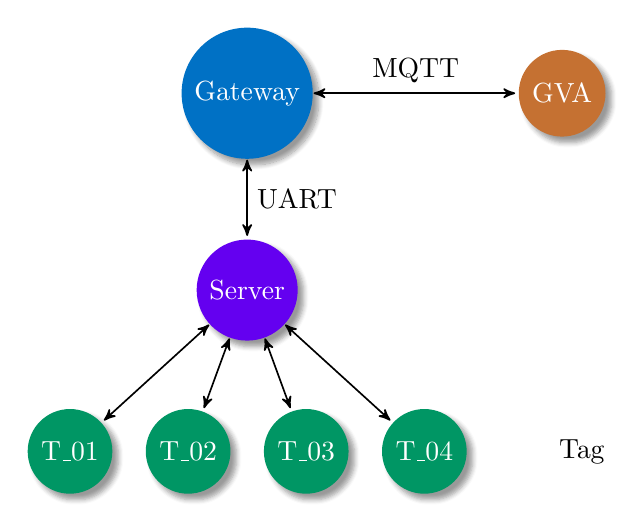
\begin{tikzpicture}[
    <->,>=stealth',shorten >=1pt,auto,node distance=5cm,semithick,
    every text node part/.style={align=center}]

    
    \node [gateway] (Gateway) {Gateway};
    
    \node [gva] (GVA) [right of = Gateway, node distance=4cm]{GVA};

    \node [server] (Server) [below of = Gateway, node distance=2.5cm]{Server}
    child{node (Client01) [leaf] {T\_01}}
    child{node (Client02) [leaf] {T\_02}}
    child{node (Client03) [leaf] {T\_03}}
    child{node (Client04) [leaf] {T\_04}};
    \node (ClientLeaf)  [right of = Client04, xshift = -3cm] {Tag};
    
    \path (Gateway) edge[]    node[] {UART} (Server);
    \path (Gateway) edge[]    node[] {MQTT} (GVA);

    
    \end{tikzpicture}
    \caption{Structure of the IoT enviroment}
    \label{fig:topology}
\end{figure}


\subsection{Tag}


The tag collects data from the sensors, establishing communication with the server and storing data in periods of disconnection with the wireless sensor network. It is a device based on a 32-bit microcontroller powered by a coin-cell battery, which communicates with different external modules as PWM controller, NFC RFID, flash memory, SRAM, cryptographic module and temperature, humidity, luminosity, and accelerometer sensors (see Fig. \ref{fig:tag}). It uses SPI and I2C protocols and has an integrated RF interface that operates in the 2.4 GHz band, with 16 channels ranging from 2.4 to 2.4835 GHz, O-QPSK modulation, and bit rate of 250 kbps per channel. The microcontroller is programmed in C language using multiple libraries supplied by microcontroller and embedded modules manufacturers, and libraries developed by the company's own development team.

\begin{figure}[t!]
\centering
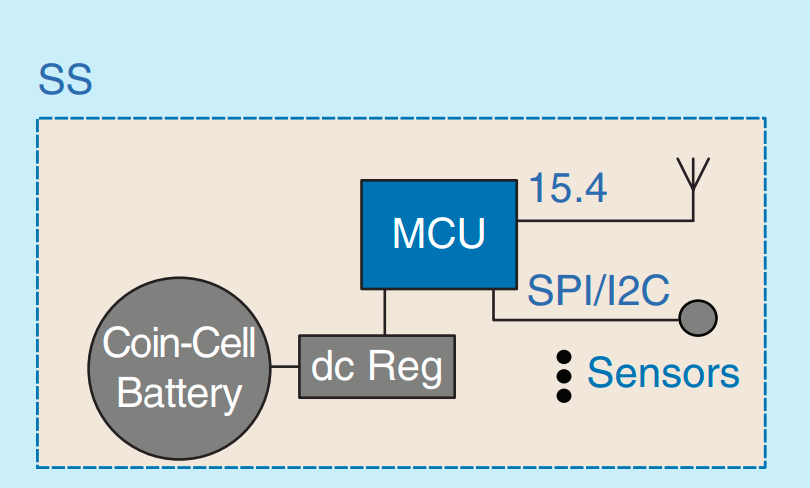
\includegraphics[width=0.9\columnwidth]{fig3.png}
\caption{Block diagram of Tag module in the IoT environment. Source: Adapted from \cite{williams2017weaving}.}
\label{fig:tag}
\end{figure}

To manage the processes that must be executed by the Tag, programming based on state machines and timed state machines was developed within it. The Tag is able to identify different events that allow it to change the operation states, programming timed tasks, and defining sleep periods in order to execute minimal instructions quickly. And only as needed, prioritizes sleep to minimize the duty cycle and the circuital current consumption. An example of state machine used for a tag is shown in Fig. \ref{fig:state_machine}, in which

\begin{figure}[!t]
\centering
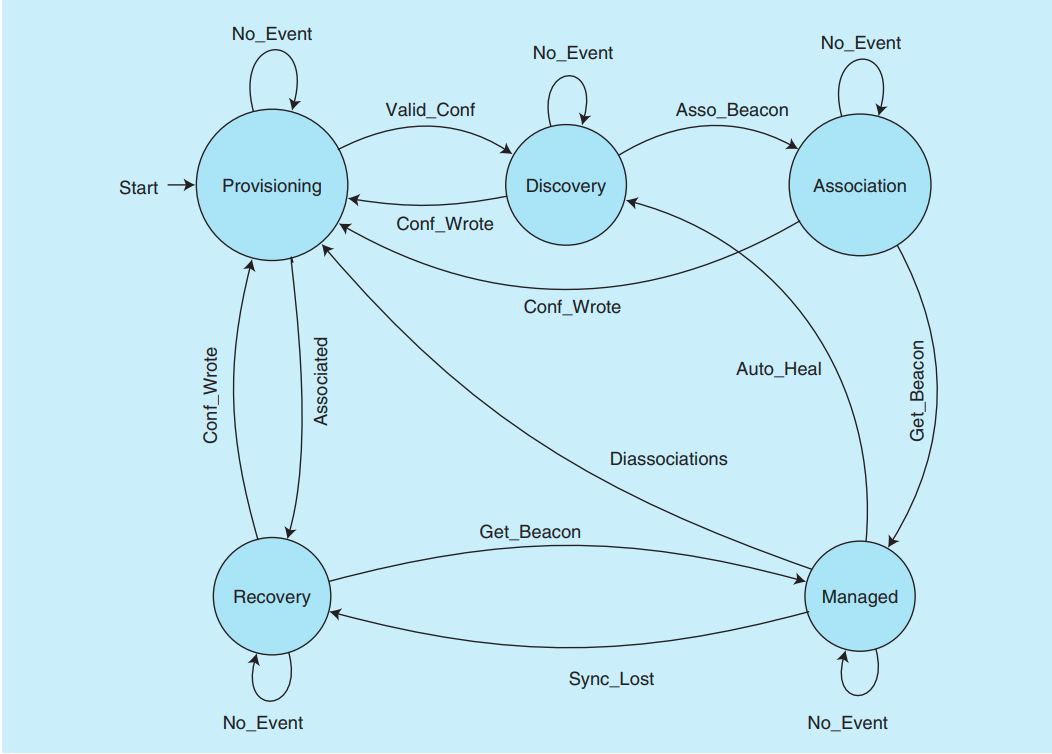
\includegraphics[width=0.95\columnwidth]{fig6.png}
\caption{Example of the management subsystem state machine used for the wireless sensor network. Source: Adapted from \cite{williams2017weaving}.}
\label{fig:state_machine}
\end{figure}

\begin{enumerate}
\item \textbf{Provisioning:} It is the initial state for a node. Its function is to wait until basic configurations are provisioned to a node for network connectivity. For example, channel and Gateway IDs, macro frame interval, sensor thresholds, etc.
\item \textbf{Association:} After the node receives the configurations in the provision state, the node must join the network. In this phase, the client is not yet synchronized, and the clients need to receive their time slot assignment from the server to form the TDM network. For this reason, the client node waits until receive from the server an association beacon with the respective time-slot.
\item \textbf{Managed:} After the association process is accomplished, the client node can work on the operations as a sensor node. That is, the node conduct routine scheduled operations according to micro/macro frame periods, using various beacons to synchronize, change configuration, report sensor data, etc.
\item \textbf{Recovery (reconnection):} If a client node loses synchronization due to radio interference or another perturbation, causing a mismatch between the server's clock reference points, it accelerates its wake-up schedule, attempting to increase the probability of receiving a beacon.
\end{enumerate}


\subsection{Unified Gateway Server}


It is a hybrid system made up of an Android device and a microcontroller-based device. These devices are called Gateway and Server, respectively.


\subsubsection{Gateway}
\label{sec:gateway}


Different applications run in this device allowing communication between the cloud and the wireless sensor network. Each of them fulfills specific tasks. The modular architecture allows distributing the task load and managing the search and troubleshooting more efficiently. Some of the functions developed by the different applications are:

\begin{enumerate}

\item Communication interface for the WSN server converting complex messages into commands, that are understandable to the server and also in the opposite direction.
\item Communication interface with the cloud for telemetry data.
\item Interface for trusty functions, such as key storage, encryption, etc.
\item Send critical diagnostic information to the cloud for troubleshooting purposes.
\item Check for software updates.
\end{enumerate}

Regarding to its components (see Fig. \ref{fig:gateway}), it is a device based on a 4-core microprocessor with Android operating system. This device is in charge of receiving information related to the tags from the server (through an UART module), processing the information, packaging it, and sending it to the cloud. It uses the standard Wi-Fi Network IEEE 802.15.4 or the cellular network. Also, this device is equipped with a GPS module, an LCD screen to display information about the connection process with the sensor network, a power indicator LED, a beeper, and a battery with a capacity of 10 to 40 days. Moreover, the Gateway is responsible for supplying energy to the server.

\begin{figure}[t!]
\centering
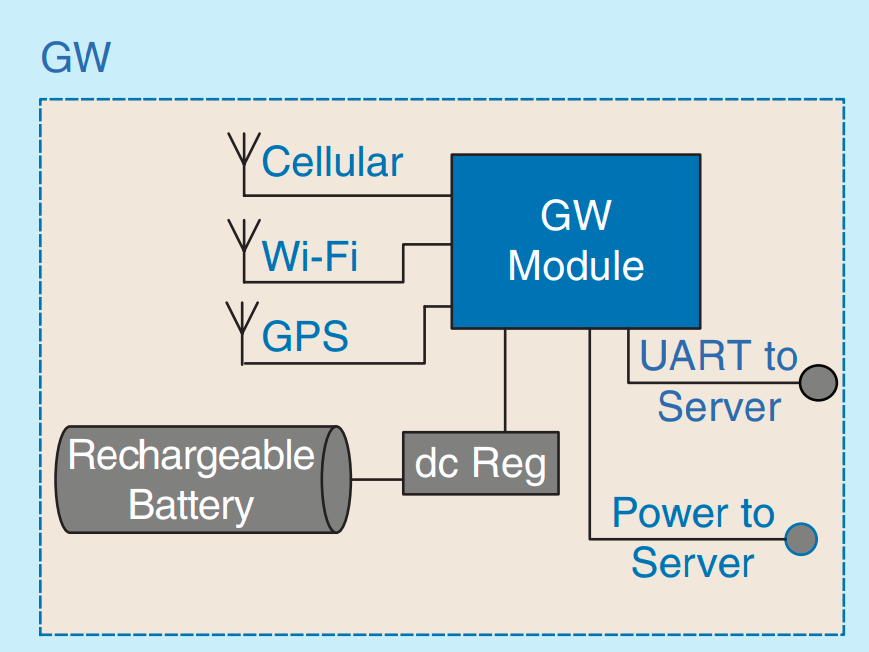
\includegraphics[width=0.9\columnwidth]{fig4.png}
\caption{Block diagram of Gateway module on the unified GW server device. Source: Adapted from \cite{williams2017weaving}.}
\label{fig:gateway}
\end{figure}


\subsubsection{Server}


Like the tag, the server is a device based on a 32-bit microcontroller, whose main purpose is to be a communication bridge between the Gateway and the tag's network. Therefore, server firmware is designed to receive and send messages to both sides. Moreover, it has a connection with different sensors like the tag and it has to be pending to retrieve data from the sensors module.

To accomplish its functions, the server has an integrated RF interface, that operates in the 2.4 GHz frequency band with the same characteristics as the tag, UART, SPI and I2C communication modules, cryptographic module, and temperature, humidity, luminosity, and accelerometer sensors. Fig. \ref{fig:server} shows the server's block diagram.

\begin{figure}[t!]
\centering
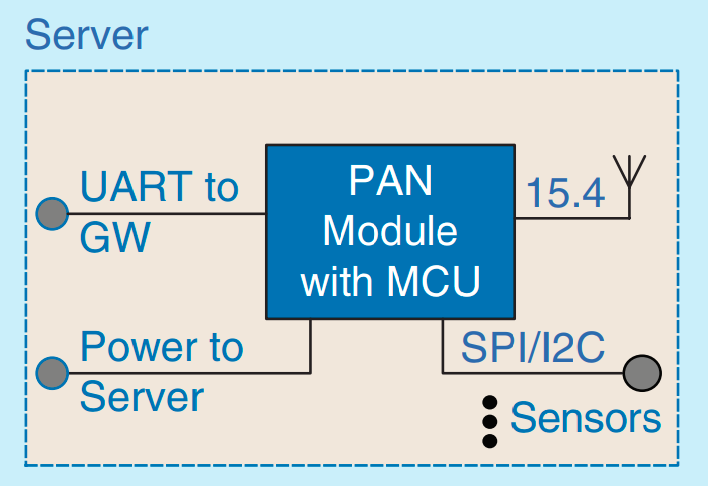
\includegraphics[width=0.9\columnwidth]{fig5.png}
\caption{Block diagrams of Server module on the unified GW server device. Source: Adapted from \cite{williams2017weaving}.}
\label{fig:server}
\end{figure}

Regarding its operation, it is important to clarify that the server has a programming logic based on state machines. Each state is designed to behave differently using a specific task list routine, and each task runs sequentially. It is shown in Fig. \ref{fig:server_tasks}.

\begin{figure}[t!]
\centering
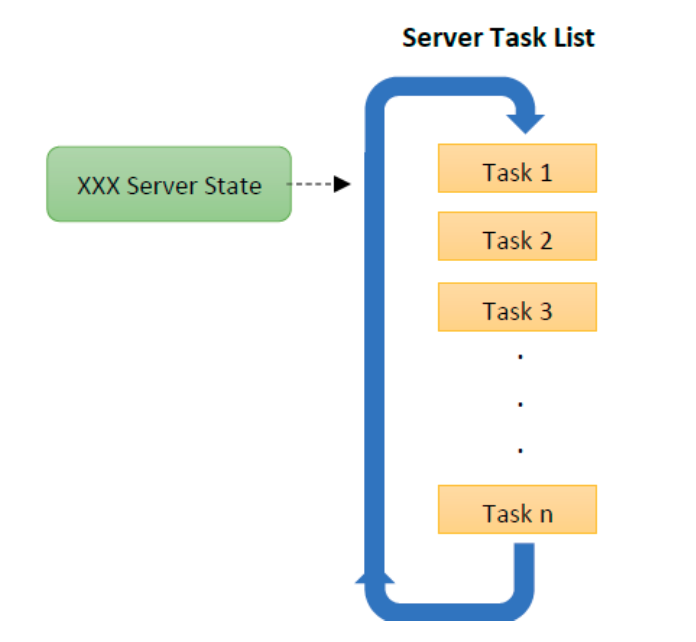
\includegraphics[width=0.8\columnwidth]{fig8.png}
\caption{Server Operation based on task list routine.}
\label{fig:server_tasks}
\end{figure}


\subsection{Gateway  Virtual  Appliance (GVA)}


The GVA is a group of modules in the cloud that communicates with the sensor network by a IoT protocol, capturing and processing messages, storing data in relational and non-relational databases, managing configuration information, operation, and capturing sensor network data, for later visualization on a web platform.


\subsection{Communication between system components}


The process of sending data between the components of the sensor network is made up of three levels. The following is a brief operation description of each of these.


\subsubsection{Tag/Server communication}
\label{sub:tag_server}


The WSN encompass N sensor nodes (tags) that connect to a receiver (server) using the IEEE 802.15.4 standard. These devices communicate by sending packets with defined structures, specific for each type of message (beacon). The structure of a message contains different fields with an assigned byte length: a header used as an identifier for the message type, configuration flags, synchronization time, system time, information about the TDM system, system parameters, and other payload data. Fig. \ref{fig:beacon_example} shows a message example.

\begin{figure}[t!]
\centering
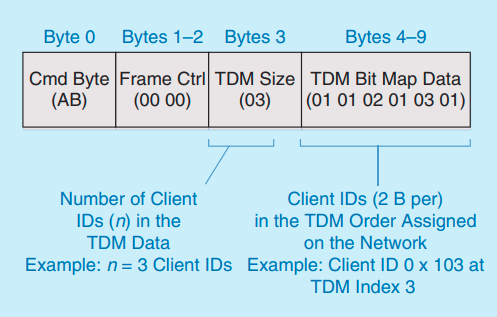
\includegraphics[width=0.9\columnwidth]{fig10.png}
\caption{A message example (beacon with AB header) for a wireless sensor network with 3 tags. Adapted from \cite{williams2017weaving}.}
\label{fig:beacon_example}
\end{figure}

Each set of tag and server device uses local timers and counters that assist them in accurate measurement of time intervals. The system has a mechanism for node clock synchronization based on the messages called "reference beacons". The reference beacon marks a "micro-frame period" initiated by the server, which allows the WSN member nodes to synchronize the clocks. With regard to receiving a beacon, all tags calculate their respective "time slots" and configure their wake-up triggers to respond with a heartbeat, or report a message in that time slot. A multiple of that period is the "macro frame period", in which tags can send additional information, such as long-term analysis data as well as errors or breaches ("anomalies").

Once the network is provisioned, all tags are anchored to the reference beacon for network management or data collection. Fig. \ref{fig:beacons} shows the operation mode for 2 tags in a network. Note that the response of client 2 is offset by a time since the beacon reception, avoiding the message crossing between clients. This operation ensures the precise separation between "time slots" because synchronization is carried out with the arrival of each reference beacon.

\begin{figure}[t!]
\centering
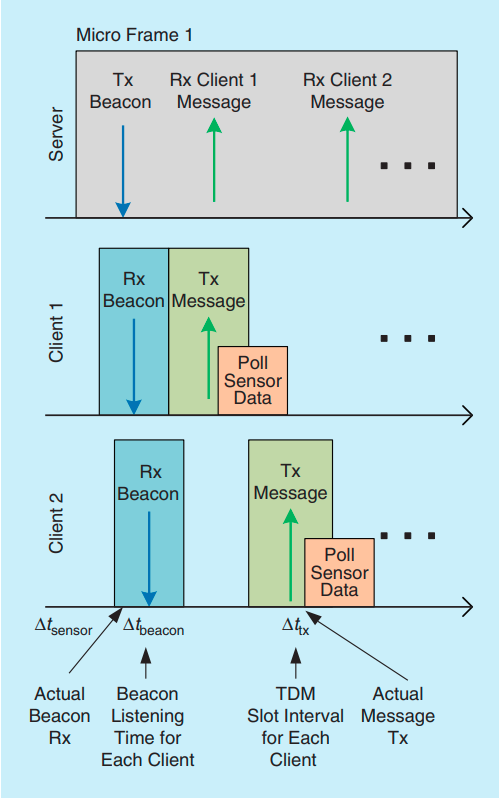
\includegraphics[width=0.8\columnwidth]{fig9.png}
\caption{Operation of a sensor network with two clients. Rx: receive, Tx: transmit. Adapted from \cite{williams2017weaving}.}
\label{fig:beacons}
\end{figure}


\subsubsection{Server/Gateway communication}


In this section the server/gateway communication is described. It is important to clarify that all the incoming data or packets, from either wireless client network or serial port, will be put into a message entry in associated interrupt handlers and be queued in a server message list. So, the server can pick up the right time to process them and will not interfere with the beacon sending and time synchronization between server and client.

The communication between these components uses the serial port, transmitting packets in the form of a byte frame, with defined headers that identify the type of message and different structures depending on the header. The payload of the messages may contain different number of bytes (length) and be related to system configurations, such as communication channel used, shipment ID, operating modes, sensor configuration parameters, as well as provisioning and association processes. 

As previously was said, the main purpose of the gateway is to serve as a bridge between the server and the cloud. For this reason, one of the gateway applications is converting the bytes received from the server into complex messages, to be sent to the cloud, as well as converting the messages received from the cloud, into an array of bytes to be sent to the server.


\subsubsection{Gateway/GVA communication}


The GVA uses the MQTT protocol to communicate with the gateway. MQTT is an standard messaging protocol for the Internet of Things (IoT). It is an extremely lightweight publish/subscribe messaging transport that is ideal for connecting remote devices, with a small code footprint and minimal network bandwidth. Currently, MQTT is used in a wide variety of industries such as automotive, manufacturing, telecommunications, oil and gas, etc. \cite{mqtt}.

The bidirectional messages between the GVA and the gateway are in the form of JavaScript Object Notation (JSON). JSON is a lightweight data exchange format. Reading and writing these messages is simple for humans, and for machines it is simple to interpret and generate them. It is based on a subset of the JavaScript programming language, but its use is independent of the development language, including low-level and high-level languages. These properties make JSON an ideal language for data exchange \cite{json}. Fig. \ref{fig:json} shows a JSON message example.

\begin{figure}[t!]
\centering
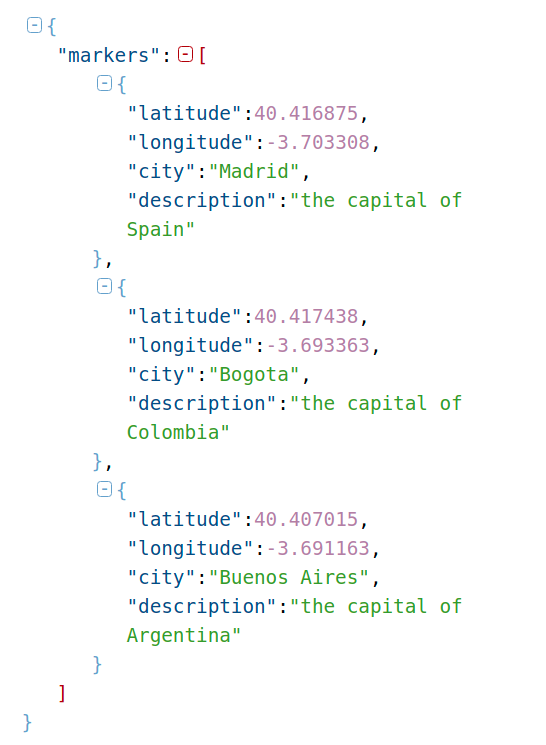
\includegraphics[width=0.8\columnwidth]{fig11.png}
\caption{JSON message example.}
\label{fig:json}
\end{figure}


\section{Description of the operation of the simulated system}


To run functional tests on component's code, TaIO Systems has developed scripts that facilitate the test compilation and running on Linux-based systems. This section describe the main characteristics of the simulation system, including the simulation mechanism for each component and the way they communicate with each other. Fig. \ref{fig:simulated-system} shows a diagram of the simulated system structure.

\begin{figure}[t!]
\centering
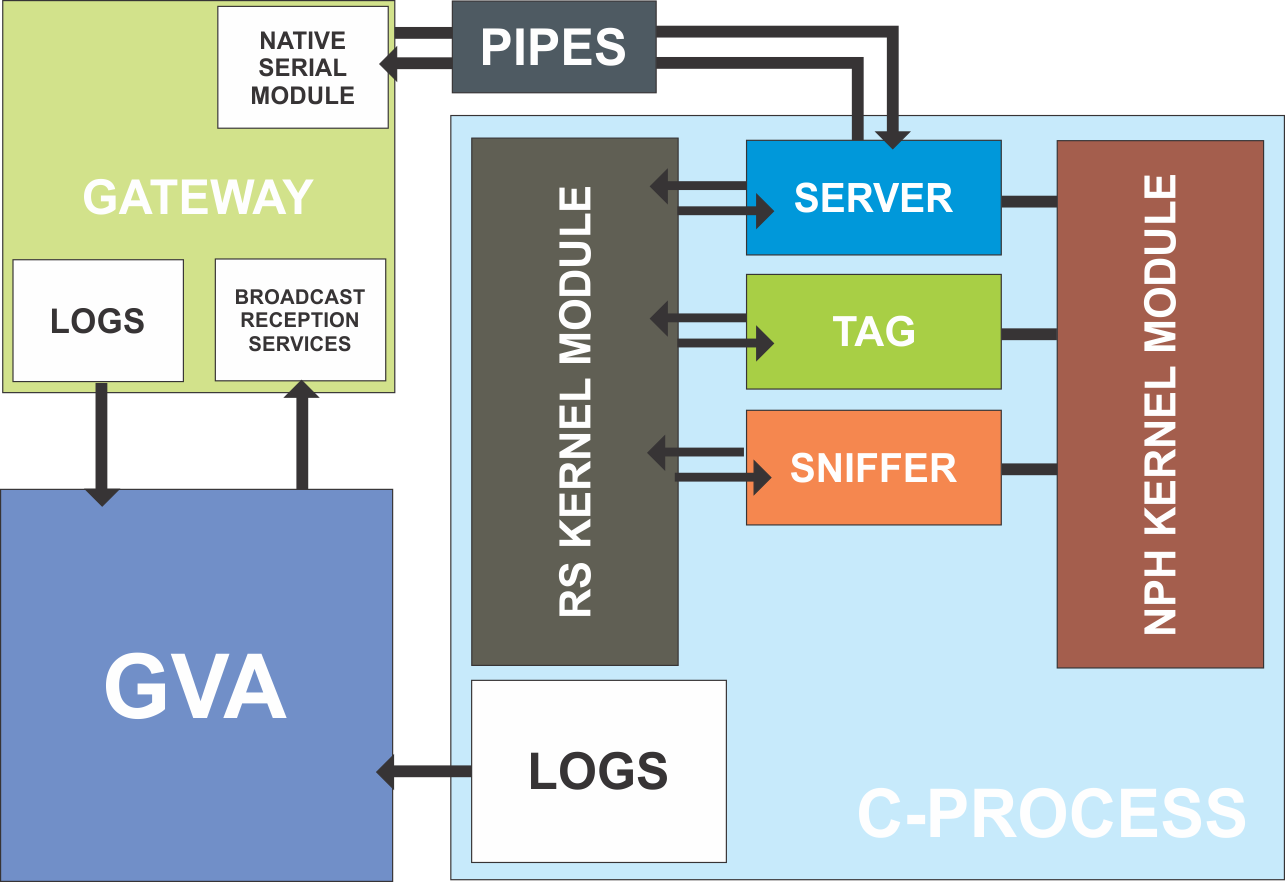
\includegraphics[width=0.95\columnwidth]{SIMULATED-SYSTEM.png}
\caption{Simulated system structure.}
\label{fig:simulated-system}
\end{figure}


\subsection{Simulated tag and server}


As mentioned above, the tag runs firmware written in the C language, which can be compiled on a Linux system using the gcc compiler, generating a binary file that can be run by the computer. For the binary to be executed correctly, it is necessary to write several scripts in order to replace the operation of different subcomponents of them. For example, flash memory, sensor response, the cryptographic module, random number generation, and the communication phase with the server.

Something important in the implementation, is the ability to switch between the simulated system's scripts and the real system by compilation flags, allowing to share most of the source code between these two modes of operation. Thus, the tag's main operation is not altered, including the handling of its state machines, timed state machines, task listing routine, and other execution routines.


\subsection{Sniffer}


It is a C script that allows us to collect the transmitted information by the communication channel, used by the server and the tags to be viewed in a readable form by the user. In the same way as the server and the tags, this script is compiled using the gcc compilation tool.


\subsection{Synchronization of multiple threads based on kernel}


For certain tests, it is enough to simulate separately each system components, but to verify functions that define more complex behaviors, it is required to simulate more than one component at the same time, for example, a server and a tag, or a server and multiple tags. In these cases, a mechanism is required that allows multiple scripts (simulated firmwares) to be executed, and their clocks need to be synchronized independently from the priority given by the computer's operating system, to each of the executed processes.

To meet this objective, we worked in the implementation of a system that allows the execution of multiple binary files resulting from the compilation of the sniffer, server and tags. Additionally, a kernel module was implemented to handle global variables, which are shared by all processes, and such as simulation time and connection/disconnection flags. This module is called the Native Process Handler Kernel Module (NPHKM).

The operation of the synchronization process consists of the execution of sections of code in each of the threads (tags/server). Each of these sections is known as "macro-task". Each of the threads executes a macro-task and sends a signal called "Yield" to the kernel module, indicating that it is ready for a next clock step. In the case of the server and the tags, a macro-task can be defined between two sleep intervals, or in a data reception, or transmission cycle. In the case of the sniffer, a macro task corresponds to an operating cycle, in which it checks for messages on the communication channel. Fig. \ref{fig:nph_kernel} shows a diagram of the kernel module's synchronization process.

\begin{figure}[t!]
\centering
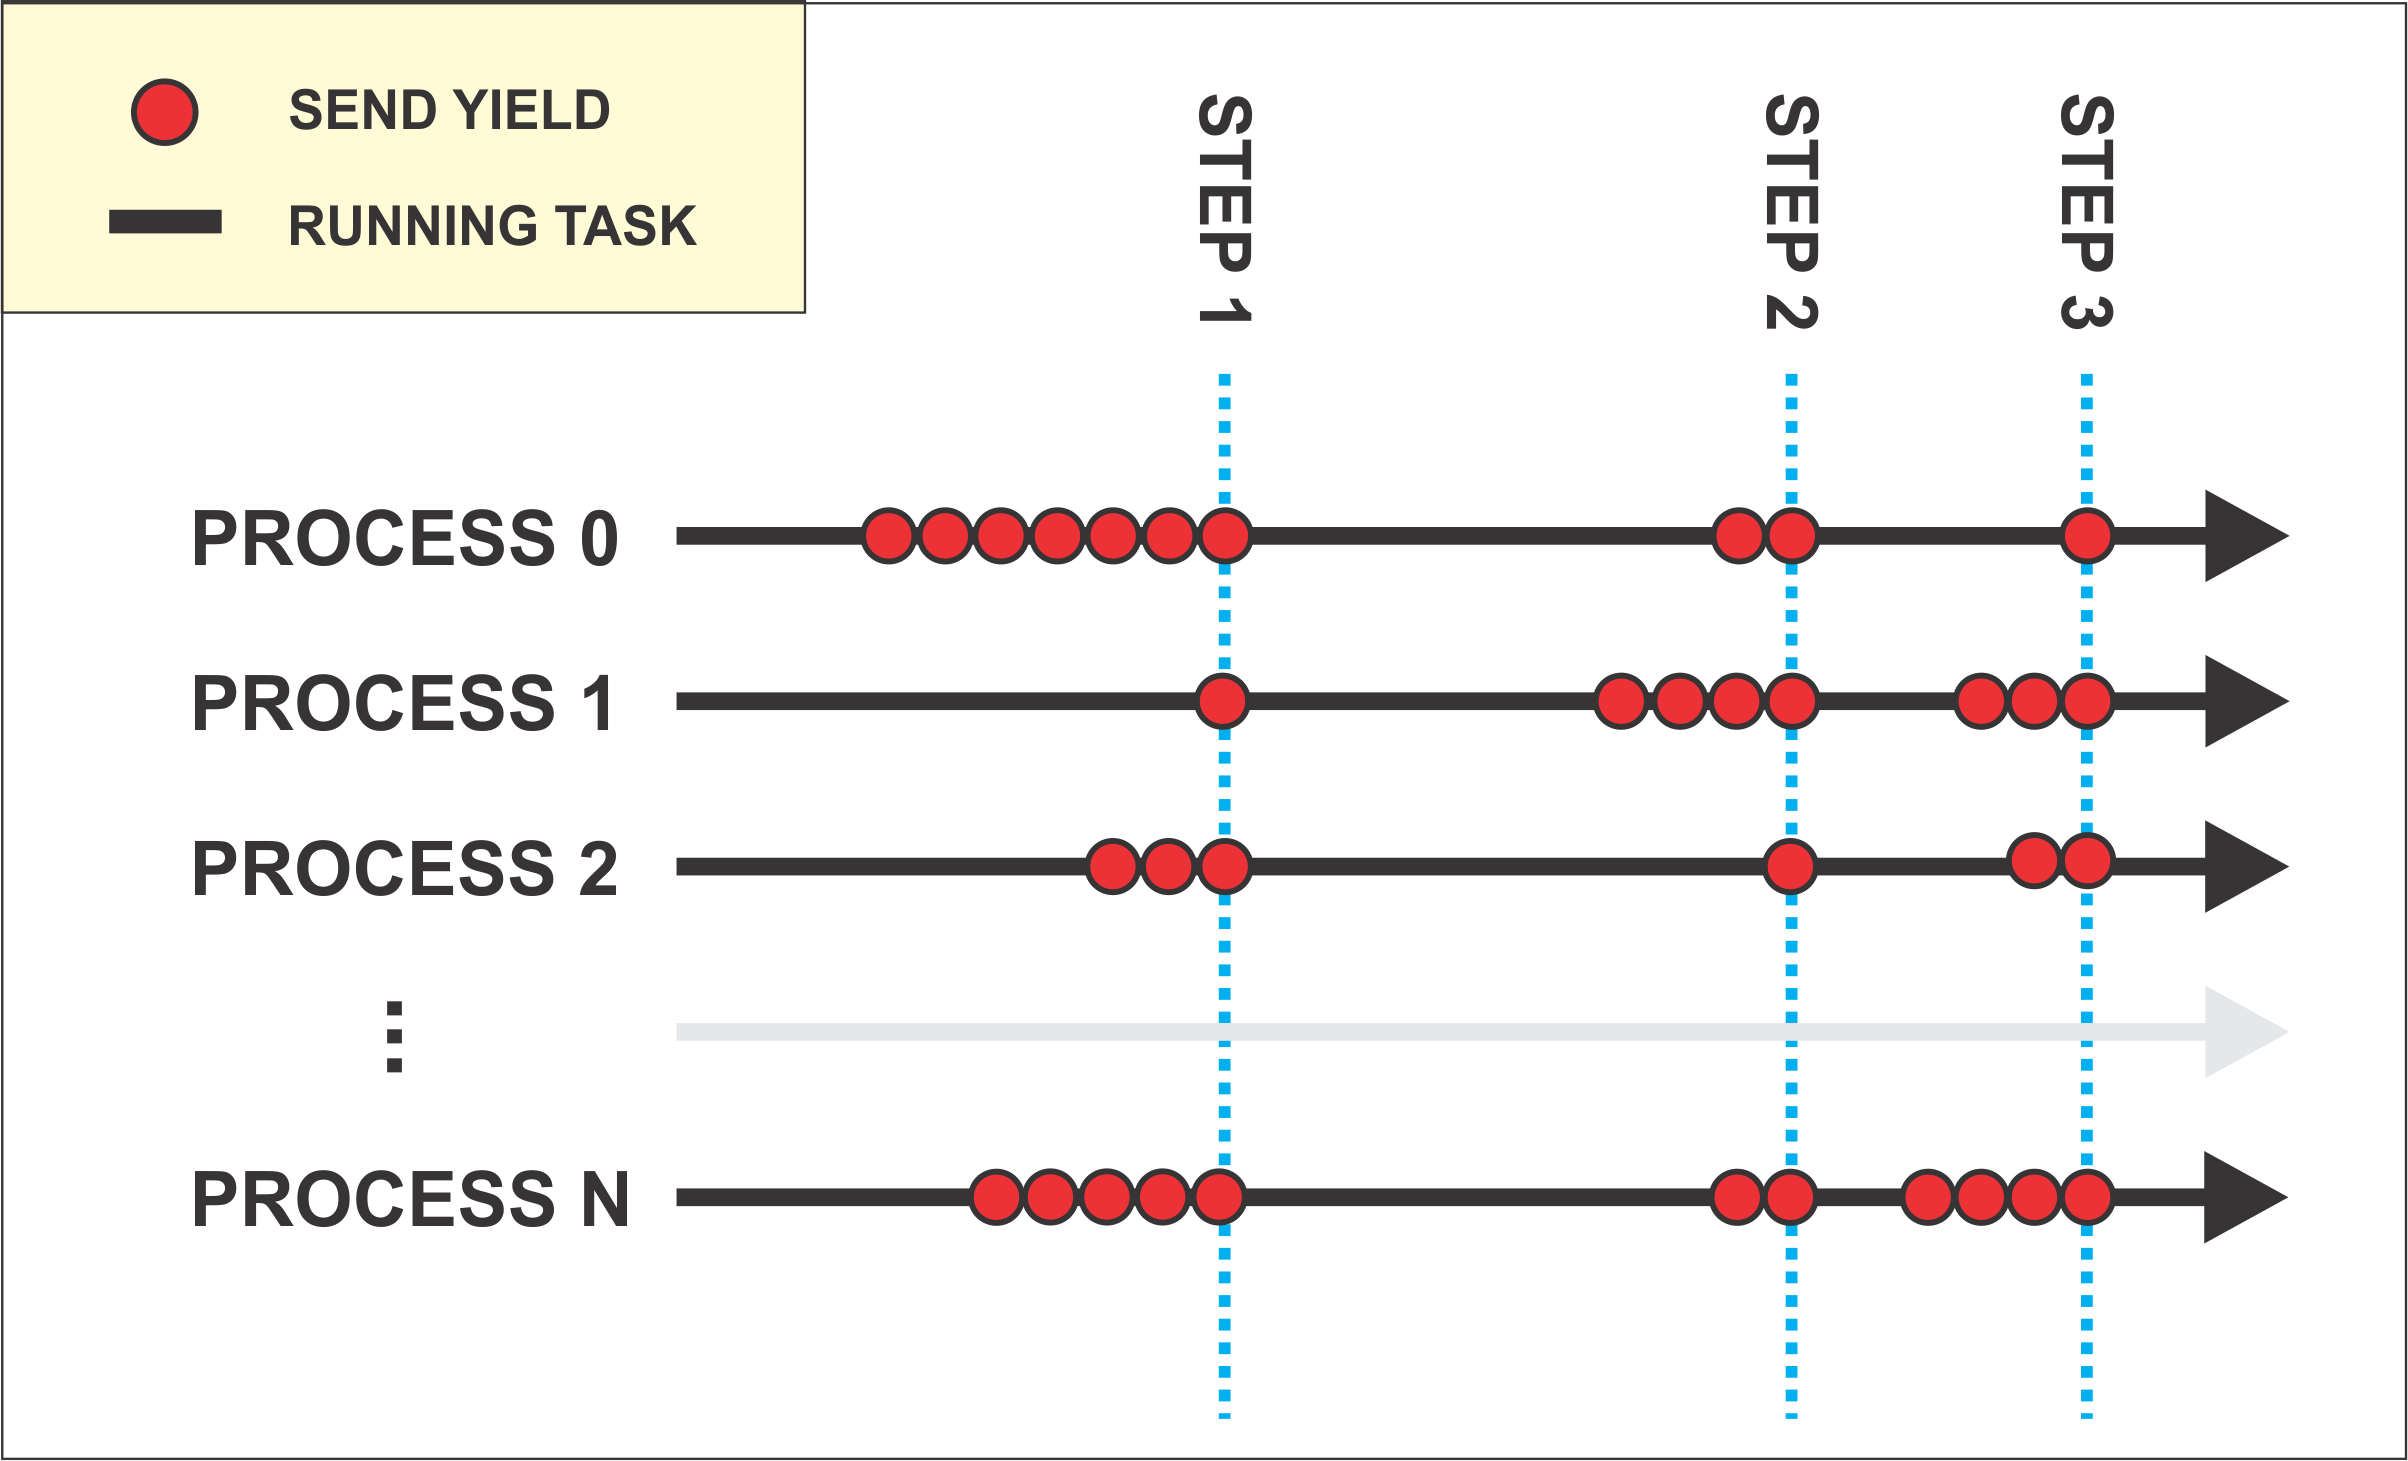
\includegraphics[width=0.9\columnwidth]{KERNEL_SYNC.png}
\caption{Synchronization process for the NPH Kernel Module.}
\label{fig:nph_kernel}
\end{figure}

All messages sent to the kernel module are transmitted in the form of an array of bytes. They are processed by a command handler, which chooses a function to be executed, based on the first byte that plays the role of header and identifier of the message. The different types of messages received by the module are:

\begin{itemize}
    \item ADD NEW PROCESS: Used to add a new subprocess identification to the thread list in the kernel module.
    \item PROCESS YIELD: Used to set the yield flag of a specific thread.
    \item SET NUMBER ACTIVE PROCESS: Used to set the number of active threads in order to know when all processes are ready for a new clock step.
    \item SET CONNECTION STATUS: Used to set the connection state of a specific thread.
    \item CLEAN: Used to clean the system clock, number of process, and flags in the kernel module.
\end{itemize}

Besides, the threads can request the kernel module for the value of the following variables:

\begin{itemize}
    \item SYSTEM CLOCK: This variable stored by kernel module in order to shared the current simulation time to the threads.
    \item CONNECTION PROCESS FLAG: This variable stored the state of connection of a thread.
\end{itemize}


\subsection{Simulated gateway}


To incorporate the operation of the gateway to the simulated system, the Android SDK is used. It includes an Android device emulator, which is a virtual device that runs on a computer, and allows Android app development and testing without using a physical device. This emulator runs a version of the gateway firmware, that covers the first function described in Section  \ref{sec:gateway}. It was not necessary to emulate the other gateway components and applications to meet the company's requirements. This Android application is compiled with the development IDE called Android Studio, which makes use of the compilation tool called gradle.


\subsection{Simulated GVA}


Due to the current gateway messages was not sent to the cloud, it was necessary to complete the fully development of this simulated system module. This module will be further explored in Section \ref{sec:Gateway-GVA}. The development of this component was carried out in Python language, making use of different free license libraries previously authorized by the company's policies. Also, this module is capable of receiving messages from the gateway, processing, validating, executing cryptographic algorithms, and providing a response to the sensor network.


\subsection{Simulation of the tag/server communication}


As mentioned in a previous section, the server and tag communicate using the IEEE 802.15.4 standard, but in the case of their simulated counterparts, these devices communicate using a kernel module called the "Radio Simulator Kernel Module" (RSKM). It works as a shared communication channel between all the threads of the simulated system, like the component behavior in a real scenario. This module allows us to store the messages received from any thread, and later send it in response to a read request.

When a new message is received by the kernel, it overwrites the previous message. This could mean a problem for a system that does not use TDM, in which messages from multiple tags would be overwritten before being read by the server. Fig.  \ref{fig:radio_kernel} shows the time diagram of this module kernel.

\begin{figure}[t!]
\centering
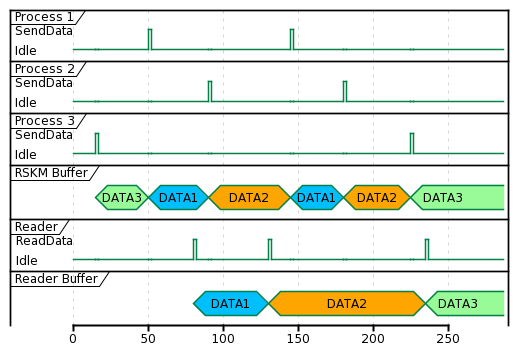
\includegraphics[width=0.98\columnwidth]{radiokernel.png}
\caption{Example of a time diagram for the radio simulator communication.}
\label{fig:radio_kernel}
\end{figure}


\subsection{Simulation of the server/gateway communication}


Unlike tag-to-server communication, server-to-gateway communication has only 2 nodes and there is no need to use a kernel module to share variables with multiple processes. This communication channel must be bidirectional and allow the transfer of information through two separate channels, such as a UART. Therefore, a FIFO (first-in-first-out) communication mechanism was used with 2 channels. It is also called pipe, which allows information to be transmitted between processes in a computer based on a file system \cite{fifo}.

The communication begins with a process that opens a temporary file on the system in write mode. Then it sends a data packet, and finally it waits for the other part of the pipeline to open the same file in read mode. The process do not continue their execution until the write/read operation has been completed. For this reason, it is necessary to create threads capable of handling the parallel communication task with the other tasks executed by the gateway and the server, like the mode that UART modules would work in a real environment. Fig. \ref{fig:pipe} shows an example of pipe communication.

\begin{figure}[t!]
\centering
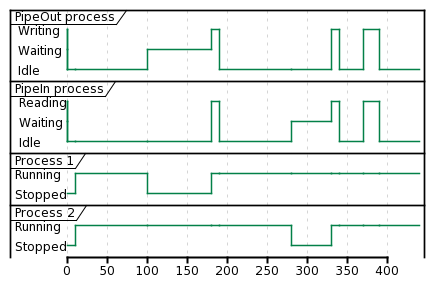
\includegraphics[width=0.95\columnwidth]{pipe.png}
\caption{Example of time diagram of the pipe communication.}
\label{fig:pipe}
\end{figure}

Since the gateway is run in the Android emulator, it is possible to simulate a serial port, passing as emulation parameter the files established for communication with pipes. Moreover, for the communication process between gateway and server to be possible, it was necessary to implement a module that simulates the device that manages the serial communication within the gateway. This module is called Native Serial Module and is composed of C++ multiple scripts, using the NDK toolset \cite{NDK}.


\subsection{Simulation of the gateway/GVA communication}
\label{sec:Gateway-GVA}


In the simulation system, the GVA is programmed in Python and must be able to receive and send JSON messages to the gateway. Therefore, a solution was established to communicate these modules and is composed of the following two sharing mechanisms.


\subsubsection{Send messages to Gateway}


Intents are used to transmit messages to the gateway. An intent is a messaging object that we can use to request an action from another component of the app, or from an external app \cite{Intents}. The emulator device is capable of receiving external intents through commands of the ADB (Android Debug Bridge) tool \cite{ADB}. These intents are received by a broadcast reception service, which is in charge of processing the information from the GVA, so the corresponding command is subsequently sent to the server. Fig.  \ref{fig:sendIntent} shows an example of an ADB command to send an intent.

\begin{figure}[t!]
\centering
\begin{lstlisting}[language=bash]
    adb shell "am broadcast -a com.example.application.jsonReciver --es JSON "{ "name": "Robert", "age": 52, "address": "Cra. 35 #15-22", "pets": ["Tasha","Molly","Blast"] }" "
\end{lstlisting}
\caption{Example of a command to sent a JSON intent.}
\label{fig:sendIntent}
\end{figure}


\subsubsection{Receive messages from Gateway}


To receive messages from the gateway, the simulated GVA uses the Logcat tool, which dumps a log of messages from the Android Device's emulation system, including stack traces, system error cases, and debugging messages, that are written from the applications \cite{Logcat}.

Debugging messages are enabled into the application executed by the GVA. Some message are written to normally be sent to the cloud in JSON format. In this way, the simulated GVA can access them, process them, and send a response back if it is necessary.


\subsection{C-Process}


Some of the components that belong to the simulation system are written in C. They are compiled with the same gcc tool, and for this reason, the simulation system has text files called makefiles, which are capable of compiling multiple C programs at the same time using variables, flags, patterns, and functions. The tool used to execute these files is called Make \cite{Make}.

A script was also implemented in order to load the server binaries, tags, sniffer, and kernel modules. And after that, it uses the native C library thread for running each of the compiled process in a different thread.


\section{Description of the Behaviour Driven Development(BDD) methodology}


BDD is a synthesis, refinement, and evolution of agile development practices derived from Test Driven Development (TDD) and Acceptance Test Driven Development (ATDD). These techniques allow the developer to be focused on the implementation of an specific task, and are essential in the Quality Assurance (QA) of software process. The concept of quality has multiple interpretations, but it always implies that the software satisfies the customer's needs. At this point, BDD becomes important and stands out to TDD and ATDD, because it allows the development of more complex test scenarios, including behaviors that other methodologies inhibit their definition.

The idea of BDD was born from the need for developers to show the results of unit tests, function tests, or sets of functions that describe the system behavior. In addition, it responds to understanding if the task to be developed had been completed with success, or if there is an error, and to identify the reason for the failure. Agiledox is a tool that was developed by Chirs Stevenson \cite{dannorth}, which allows to extract the names of the unit tests from testing tools like JUnit, and print them as sentences. An example developed with this tool is shown in Fig.  \ref*{fig:JUnitTest} and Fig. \ref*{fig:agiledox}.

\begin{figure}[t!]
\centering
\begin{lstlisting}[language=java]
    public class CustomerLookupTest extends TestCase {
        testFindsCustomerById() {
            ...
        }
        
        testFailsForDuplicateCustomers() {
            ...
        }
        ...
    }
\end{lstlisting}
\caption{Example of the JAVA JUnit test.}
\label{fig:JUnitTest}
\end{figure}

\begin{figure}[t!]
\centering
\begin{lstlisting}[language=Matlab]
    CustomerLookup
    - finds customer by id
    - fails for duplicate customers
    - ...
\end{lstlisting}
\caption{Agiledox result.}
\label{fig:agiledox}
\end{figure}

The word "test" is stripped from both the class name and the method names, and the camel-case writing is transform in the regular text. This tool is also used by programmers to obtain software documentation files, naming their unit tests with statements that describe the purpose, and even using commercial language to share test results with other company's members and customers.

In \cite{north2010introducing}, Dan North proposes a new strategy that emphasizes in solving the aforementioned problem. It modifies the vocabulary used to define the tests clarifying the purpose of behavior-based development, basing this structure on a ubiquitous language to describe the requirements of the software tests. And finally, it defines them in the form of test scenarios. The structure or template that defines a BDD scenario has the following form:

\begin{enumerate}
    \item \textbf{Given} some initial context (the givens),
    \item \textbf{When} an event occurs,
    \item \textbf{Then} ensure some outcomes. 
\end{enumerate}

Besides, the developer can use the extra word "And" in order to extend the "given", "when", or "then" sentences. Here is a classic example in which a customer wants to withdraw cash from an ATM. The software developer wants to evaluate the ATM's performance in different scenarios. For this example, some possible scenarios to be evaluated are described in Fig.\ref{fig:ATMscenario1} and Fig. \ref{fig:ATMscenario2}.

\begin{figure}[t!]
\centering
\begin{lstlisting}[]
    Scenario 1: Account is in credit

        Given the account is in credit
        And the card is valid
        And the dispenser contains cash
        When the customer requests cash
        Then ensure the account is debited
        And ensure cash is dispensed
        And ensure the card is returned
\end{lstlisting}
\caption{ATM BDD Scenario 1.}
\label{fig:ATMscenario1}
\end{figure}

\begin{figure}[t]
\centering
\begin{lstlisting}[]
    Scenario 2: Account is overdrawn past the overdraft limit

        Given the account is overdrawn
        And the card is valid
        When the customer requests cash
        Then ensure a rejection message is displayed
        And ensure cash is not dispensed
        And ensure the card is returned
\end{lstlisting}
\caption{ATM BDD Scenario 2.}
\label{fig:ATMscenario2}
\end{figure}

Both scenarios are based on the same event and have some givens and outcomes in common. With this structure, we can re-use givens, events, and outcomes. When multiple scenarios are focused on the verification of a particular system characteristic, they are organized in features. For the above mentioned example, a feature could be the one shown in Fig. \ref{fig:ATMfeature}.

\begin{figure}[t!]
\centering
\begin{lstlisting}[]
   Title: Customer withdraws cash
    
    As a customer,
    I want to withdraw cash from an ATM,
    so that I don't have to wait in line at the bank.
    
     Scenario 1: ...
     ...
    
     Scenario 2: ...
     ...
\end{lstlisting}
\caption{ATM feature example.}
\label{fig:ATMfeature}
\end{figure}

This scenario writing mode (in natural language) allows a clearer description of situations to be tested, expected behaviors, and the meaning of a failure during the process. Each of these statements is linked to a function that is executed and verified. The language used to code each function is independent of the development methodology. Some multiple libraries and tools allow the incorporation of BDD in different languages, developed by companies, or communities of programmers.


\section{Description of the implementation of scenarios for the simulated system}


Currently, the IoT environment developed by TaIO System, is in the support and bug correction phase. For this reason, an automatic behavioral testing system was implemented, that aims at quality assurance of the different device firmwares. To carry out this implementation, the following phases were fulfilled.


\subsection{Selection of the BDD library}


An important part when developing software for a company is the selection and use of tools, libraries, and any third-party code. A review of different libraries for the BDD methodology implementation was done, and one of them was chosen based on different technical parameters that are described below. Table \ref{tab:libraries} shows the explored libraries.

\begin{table}[h!t!]
\renewcommand{\arraystretch}{1.25}		% Incrementa un poco la altura de las filas
\centering
\caption{BDD Libraries}	% Los rótulos deben ir arriba de la tabla
\label{tab:libraries}
\begin{tabular}{l|l|l|l}					% {l|l} define la alineación de las columnas y la línea divisoria
\hline \hline
\textbf{Library}        				&   \textbf{Developers}     &	\textbf{Language}	&	\textbf{License}			\\
\hline
Cucumber-JVM        &   SmartBear	            &	Java            &   BSD\\
Cucumber-CPP        &   SmartBear	            &	C++             &   MIT\\
Cucumber-Android    &   SmartBear	            &	Java/Kotlin     &   MIT\\
Behave              &   SmartBear/Thirdy-Party	&	Python          &   BSD\\
Jbehave             &   Jbehave	                &	Java            &   BSD\\
Specflow            &   SmartBear	            &	NET/C chart     &   BSD\\
pytest-bdd          &   Thirdy-Party	        &	Python          &   MIT\\
Radish              &   Thirdy-Party	        &	Python          &   MIT\\
\hline \hline
\end{tabular}
\end{table}

In a business environment, in which software is developed in order to sell and distribute it to third parties, it is important to ensure that the terms of the license allow this action without problems. In the case of the listed libraries, the licenses are BSD and MIT type. Both grant permission, without charge, to anyone who obtains a copy of this software and the associated documentation files. Users can operate without restrictions, copy, modify, and distribute this software for any purpose with or without a fee.

The choice of a language in which the behavioral testing system will be implemented is of utmost importance. The difficulty and time of its incorporation into the simulation system may be affected. In the IoT environment there are multiple processes running in different programming languages and communicating through multiple channels. But the processes of authorization, linking, configuration, and verification of sensor data are carried out in the highest level component: the GVA. For this reason, sharing the same language with this component, ensures easy integration with the simulation system. Based on the above criteria, 3 options are available: Behave, Pytest-BDD, and Radish.

In the last stage of selection, the stability of the software to be integrated is taken into account. Adding a library that contains bugs, plus to a small support team, could translate into an increase in development time. Thus, a development company with a large team, capable of supporting and updating the tool, contributes to the stability of the parent software that use the library.

Based on these 3 selection criteria, the most convenient option is the Behave library, which is supported by the SmartBear Company, with contributions from the programmer community that is using it \cite{behave2021github}.


\subsection{Automation of the simulated system execution process}


For the behavioral testing system, a requirement is that the simulated system's compilation and execution must be done in an automated way, before starting to execute the BDD scenarios. Therefore, a Python script is implemented with functions aimed at compiling and executing sequentially each component. A function list and the execution order is described:

\begin{enumerate}
    \item Compile the Gateway application.
    \item Compile the C-Process with makefiles.
    \item Clone the binary file of simulated tag (if it is necessary).
    \item Make a FIFO to server/gateway communication.
    \item Run Android emulator.
    \item Install the Gateway application.
    \item Run the C-Process.
    \item Run the Gateway application.
    \item Bind Logcat output to a document.
\end{enumerate}

Step 3 is only necessary when you want to run multiple tags in the simulation system.


\subsection{Integration of the library to the simulated system}


With a library to implement BDD scenarios and a mechanism to run the simulation system in an automated way, the Behave library was integrated into the simulation system. This section shows details about the structure of files and folders that is  necessary for compiling the scenarios with this library.


\subsubsection{Behave project structure}

Behave requires a specific file structure for the organization of the features, scenarios, steps, and auxiliary files that are used for behavioral testing. First, we set the main folder of our project, which must contain a folder called features. This folder contains a list of different features that we need to test. Then, each feature is located into a Python file, in which it is described and the corresponding scenarios are defined. Also, the feature folder must contain a folder called steps, in which there are different scripts with the definition of all the functions that execute the scenarios, i.e., the translation of the Give, When, and Then sentences into the programming language. Fig. \ref{fig:dirtree1} shows an example of this structure.

\begin{figure}[t!]
    \dirtree{%
    .1 \textbf{behaveProject}.
    .2 \textbf{features}.
    .3 environment.py.
    .3 example1.feature.
    .3 example2.feature.
    .3 *********.
    .3 exampleN.feature.
    .3 \textbf{steps}.
    .4 common-steps.py.
    .4 example2-steps.py.
    .4 *********.
    .4 exampleN-steps.py.
    .3 \textbf{utils}.
    .4 auxiliaryScript1.py.
    .4 auxiliaryScript2.py.
    .4 *********.
    .4 auxiliaryScriptM.py.
    }
    \caption{Behave file structure example.}
    \label{fig:dirtree1}
\end{figure}

The enviroment.py file is used to configure functions that run before or after a group of features or scenarios. Finally, a folder named utils stores the auxiliary scripts that are necessary for the functionality of the tests.


\subsubsection{Running a sample scenario for the simulated system}


A feature was implemented in order to verify that the simulated system successfully and automatically executes each of its components from a BDD scenario. See Fig. \ref{fig:simsys}.

\begin{figure}[t!]
\centering
\begin{lstlisting}[]
 Feature: Run the simulated system

   - As a developer,
   - I want to run all the components of the simulated system,
   - so that I don't have to compile and run each process manually.


   Scenario: All the scripts are already to compile and run without errors

    Given all the scripts are already to compile 
    When I compile and run the Gateway, server and tag
    Then I should have a simulated system running successfully
\end{lstlisting}
\caption{Test feature for the simulated system.}
\label{fig:simsys}
\end{figure}

The implemented scenario describes the procedure to be tested at a high level. In this case, it is assumed that we have all the tag, server, sniffer, kernels, and gateway application scripts, and we proceed to compile and run all the processes. The latter means executing all the automation steps of the simulation that was described in the previous section. It is expected to get the whole system working correctly. In this last step, it is verified that each of the components are running and the communication between them is working in a correct way. Fig. \ref{fig:behaveOK} and Fig. \ref{fig:behaveBAD} show the output obtained after running the scenario with Behave.

\begin{figure}[t!]
\centering
\begin{lstlisting}[style=okstyle]
Feature: Run the simulated system 
    *# features/example.feature:1*
  - As a developer,
  - I want to run all the components of the simulated system,
  - so that I do not have to compile and run each process manually.

  Scenario: All the scripts are already to compile and run without errors  
  *# features/example.feature:8*
    @Given all the scripts are already to compile@                           
    *# features/steps/example_steps.py:29 0.000s*
    @When I compile and run the Gateway, server and tag@                    
    *# features/steps/example_steps.py:33 65.580s*
    @Then I should have a simulated system running successfully@             
    *# features/steps/example_steps.py:43 5.034s*

&1 feature passed, 0 failed, 0 skipped&
&1 scenario passed, 0 failed, 0 skipped&
&3 steps passed, 0 failed, 0 skipped, 0 undefined&
Took 1m15.348s
\end{lstlisting}
\caption{Behave output for the scenario without errors.}
\label{fig:behaveOK}
\end{figure}

\begin{figure}[t!]
\centering
\begin{lstlisting}[style=okstyle]
Feature: Run the simulated system 
    *# features/example.feature:1*
    - As a developer,
    - I want to run all the components of the simulated system,
    - so that I do not have to compile and run each process manually.

    Scenario: All the scripts are already to compile and run without errors  
    *# features/example.feature:8*
    @Given all the scripts are already to compile@                          
    *# features/steps/example_steps.py:29 0.000s*
    @When I compile and run the Gateway, server and tag@                     
    *# features/steps/example_steps.py:33 65.580s*
    <Then I should have a simulated system running successfully>         
    *# features/steps/example_steps.py:43 5.034s*
    [Assertion Failed: Simulated Tag is not running]

Failing scenarios:
    features/example.feature:8  All the scripts are already to compile and run without errors
    
[0 features passed, 1 failed, 0 skipped]
[0 scenarios passed, 1 failed, 0 skipped]
[2 steps passed, 1 failed, 0 skipped, 0 undefined]
Took 1m10.614s
\end{lstlisting}
\caption{Behave output for the scenario with errors.}
\label{fig:behaveBAD}
\end{figure}

The results allow us to verify if the scenario was passed successfully or failed, and if there is a failure. It also shows the step that has a problem, and generates a general report of the scenario execution, including the time it took.


\section{Definition and development of the scenarios for the simulated system}


The previous section showed the implementation result of an example of scenario that ensures the simulation system is ready for compilation and execution. But this is only the first step to complete the objective of this work. In addition, several characteristics of relevant importance were defined to be verified for the TyIO System's team, in order to ensure that the system behaves correctly under different conditions. These features are:\\

\begin{itemize}
    \item IoT environment working with a single tag.
    \item IoT environment working with multiple tags.
    \item IoT environment working in the presence of packet loss.
    \item IoT environment facing periods of disconnection.
    \item IoT environment working in the presence of unauthorized tags.
\end{itemize}

The first and second of them represent the behavior of the system with a single tag and multiple tags respectively. In this case, the test tool has to be able to verify that the system can satisfactorily provide, associate, and configure the tags, and to guarantee the data packets reception in the GVA with the information from the sensors.

In the early project stages, the development team had to deal with the loss of packets in the communication channel, between  the server and tags. Therefore, they implemented a packet retransmission routine in order to reduce the probability of information loss and tag's de-synchronization. For this reason, it was decided to implement a third feature, in which a series of scenarios corroborate that into the firmware current version the system works satisfactorily.

This behavior is evidenced in different circumstances of a real environment. For example, those realted to high noise levels or interference in the communication channel and distance between tags and server. The distance between tag and server is highly variable in real environments, because companies that use the package tracking system cannot ensure the tags stay at a specific distance from the server. Later, we will present an analysis of the relationship between the distance of these components and the percentage of packet loss.

Another very interesting system feature is the tag ability to store the sensor captures in long periods of disconnection. During a disconnection period, the tag stores the data from the sensors in flash memory every macro-interval. When the tag instructs to connect to the server again, the tag informs that it has stored data that has not been sent yet. Then, the server sends a special message to retrieve data by data. This situation occurs frequently in a real scenario, in freight transport companies, because at the route paths the packages must be transported by plane or boat. The regulations applied to the project keep the radio communication devices turned on under these conditions, but without sending packets. For this reason,  tags must store all the data captured from the sensors even after landing. Then, it should establish connection in the presence of a gateway-server, and finally send all the stored information.

The last characteristic refers to scenarios in which multiple tags try to connect to the system, sending association messages to the server, but not all have authorization to establish connection. This situation occurs only when some of the tags have been registered in the GVA as part of a shipment.


\subsection{Packet loss and tag-server distance}


The IEEE 802.15.4 PHY layer is responsible for the transmission and reception of information through the radio channel used by the server and the tag. This standard can work in different frequency ranges, but the IoT environment hardware uses the 2,450 Mhz band, because it can be operated over all the world, unlike the 868 Mhz and 915 Mhz bands that are used and regulated in Europe and North America respectively. This layer offers a maximum data rate of 250 Kbps and is based on direct sequence spread spectrum (DSSS) technology, employing offset quadrature phase-shift keying (O-QPSK) modulation. There are 16 communication channels available in the 2,450 MHz range and each channel has 5 MHz bandwidth.

The packets in 2,450 MHz PHY operation contain a 5-byte long sync header and a 1-byte long PHY header. These fields are followed by a PHY payload with variable length (up to 127 bytes) \cite{ieee154}. A byte is made up of 2 symbols of 4 bits and each symbol is translated into a 32-bit long quasi-orthogonal pseudo-random noise (PN) sequence. Table \ref{tab:32chip} summarize these sequences.

\begin{table}[t!]
    \renewcommand{\arraystretch}{1.25}		% Incrementa un poco la altura de las filas
    \centering
    \caption{32-chip PN Sequences for 4-bit symbols. Source \cite{goyal2010evaluating}}	% Los rótulos deben ir arriba de la tabla
    \label{tab:32chip}
    \begin{tabular}{l|l|l}					% {l|l} define la alineación de las columnas y la línea divisoria
    \hline \hline
    \vtop{\hbox{\strut \textbf{Chip sequence}}\hbox{\strut \textbf{number}}}        				&   \vtop{\hbox{\strut \textbf{Data symbol}}\hbox{\strut \textbf{b0 b1 b2 b3}}}     &	\textbf{Chip sequence c0 c1 ... c30 c31}\\
    \hline
    1        &   0000	            &	11011001110000110101001000101110\\
    2        &   1000	            &	11101101100111000011010100100010\\
    3        &   0100	            &	00101110110110011100001101010010\\
    4        &   1100	            &	00100010111011011001110000110101\\
    5        &   0010	            &	01010010001011101101100111000011\\
    6        &   1010	            &	00110101001000101110110110011100\\
    7        &   0110	            &	11000011010100100010111011011001\\
    8        &   1110	            &	10011100001101010010001011101101\\
    9        &   0001	            &	10001100100101100000011101111011\\
    10       &   1001	            &	10111000110010010110000001110111\\
    11       &   0101	            &	01111011100011001001011000000111\\
    12       &   1101	            &	01110111101110001100100101100000\\
    13       &   0011	            &	00000111011110111000110010010110\\
    14       &   1011	            &	01100000011101111011100011001001\\
    15       &   0111	            &	10010110000001110111101110001100\\
    16       &   1111	            &	11001001011000000111011110111000\\
    \hline \hline
    \end{tabular}
\end{table}

The PN-bits concatenated from multiple consecutive symbols are modulated onto the carrier using O-QPSK, with odd-indexed chips modulated onto the quadrature-phase carrier, and even-indexed chips being modulated onto the in-phase carrier. On the receiver the process followed is the opposite.

The received signal is demodulated to obtain the bit stream belonging to one of the 32-bit sequences. Each sequence is compared with the possible values of the PN table and the one with the smallest bit difference is chosen, to later be translated into a symbol. This allows to correctly recognize the symbols that have been transmitted with the less difference between the transmitted sequence and the received sequence. Besides, any error in identifying the transmitted symbols is likely to be identified when the packet checksum is calculated and compared with the checksum carried in the packet header.

A valid chip sequence differs from others sequences in at least 12 and up to 20 positions. For this reason, errors that contain 5 or less bits between the transmitted and received sequence can always be corrected, and conversely, errors that contain 26 or more bit errors can never be corrected \cite{goyal2010evaluating}. In \cite{goyal2010evaluating}, a calculation of the probability of obtaining a symbol error is performed. Table \ref{tab:probability} shows these probabilities for the IEEE 802.15.4 PHY.

\begin{table}[t!]
    \renewcommand{\arraystretch}{1.25}		% Incrementa un poco la altura de las filas
    \centering
    \caption{The probability of symbol error in IEEE 802.15.4 PHY. Source \cite{goyal2010evaluating}}	% Los rótulos deben ir arriba de la tabla
    \label{tab:probability}
    \begin{tabular}{l|l}					% {l|l} define la alineación de las columnas y la línea divisoria
    \hline \hline
    \textbf{The number of chip errors}        &    \textbf{Probability of symbol error}\\
    \hline
    5 and less          &   0\\
    6                   &   0.0020\\
    7                   &   0.0134\\
    8                   &   0.0523\\
    9                   &   0.1498\\
    10                  &   0.3479\\
    11                  &   0.6496\\
    12                  &   0.9156\\
    13                  &   0.9968\\
    14 and more         &   1\\
    \hline \hline
    \end{tabular}
\end{table}

The bit error probability for an O-QPSK modulated signal under additive white gaussian noise (AWGN) is given by \cite{wComs2}.

\begin{IEEEeqnarray}{rCl}
    B &=& \frac{1}{2}erfc(\sqrt{\gamma}) \quad \text{,}
\end{IEEEeqnarray}

where $erfc$ is the complementary error function and $\gamma$ is the signal-to-noise ratio (SNR). If $B$ is the probability of receiving a bit with error, and $P_{symerr(n)}$ is the symbol error probability when $n$ chips are received, as they are  shown in the Table \ref{tab:probability}, then, the probability of interpreting an incorrect symbol is

\begin{IEEEeqnarray}{rCl}
    S &=& \sum_{n=1}^{32} \binom{32}{n}B^{n}(1-B)^{32-n}\times P_{symerror}(n) \quad \text{.}
\end{IEEEeqnarray}

A packet containing any symbol in error is considered a packet received in error. Therefore, the probability $P$ of receiving an error packet, in a transmission of packets of $m$-length bytes (or $2m$ symbols), is

\begin{IEEEeqnarray}{rCl}
    P &=& 1 - (1-S)^{2m} \quad \text{.}
\end{IEEEeqnarray}

Although a correspondence between the bit error rate (BER) and the SNR is easily understood within an engineering context, and when it is explaining and describing the test scenarios, it is important to find a relationship with a variable that is used in a business language. For this reason, the relationship between the SNR and the separation distance between two transmission points is described in the following.

The Friis transmission formula is used in telecommunications engineering. It computes the power at the terminals of a receive antenna as the product of the power density of the incident wave and the effective aperture of the receiving antenna. It takes into account idealized conditions given another antenna transmitting a known power \cite{wComs}. The Friss transmition equation is given by

\begin{IEEEeqnarray}{rCl}
    \frac{P_{r}}{P_{t}} &=& D_{t} D_{r}(\frac{\lambda }{4\pi d})^2  \quad \text{,}
\end{IEEEeqnarray}

where $P_{r}$ is the received radio wave power, $P_{t}$ is the transmitted radio wave power, $D_{t}$ is the directivity of the transmitting antenna, $D_{r}$ is the directivity of the receiving antenna, $\lambda$ is the signal wavelength, and $d$ is the distance between the antennas. Then the received power and SNR can be defined as

\begin{IEEEeqnarray}{rCl}
    P_{r} &=& P_{t} D_{t} D_{r}(\frac{\lambda }{4\pi d})^2  \quad \text{,}
\end{IEEEeqnarray}

and

\begin{IEEEeqnarray}{rCl}
    \gamma &=& \frac{P_{r}}{P_{noise}}  \quad \text{.}
\end{IEEEeqnarray}

Based on the previous analysis, the dependence between the probability of error in the transmission of $m$ bytes and the distance between a radio link (tag and server) can be calculated. To illustrate the dependence between these variables, Fig. \ref{fig:snr} and Fig. \ref{fig:distance} show the graphs for packet transmission using and not using spread spectrum (PN sequences). It assumes isotropic antennas, constant noise power, and constant transmit power, which is used by the radio link in a real scenario. Table \ref{tab:variables} shows the values of these constants.

\begin{figure}[t!]
\centering
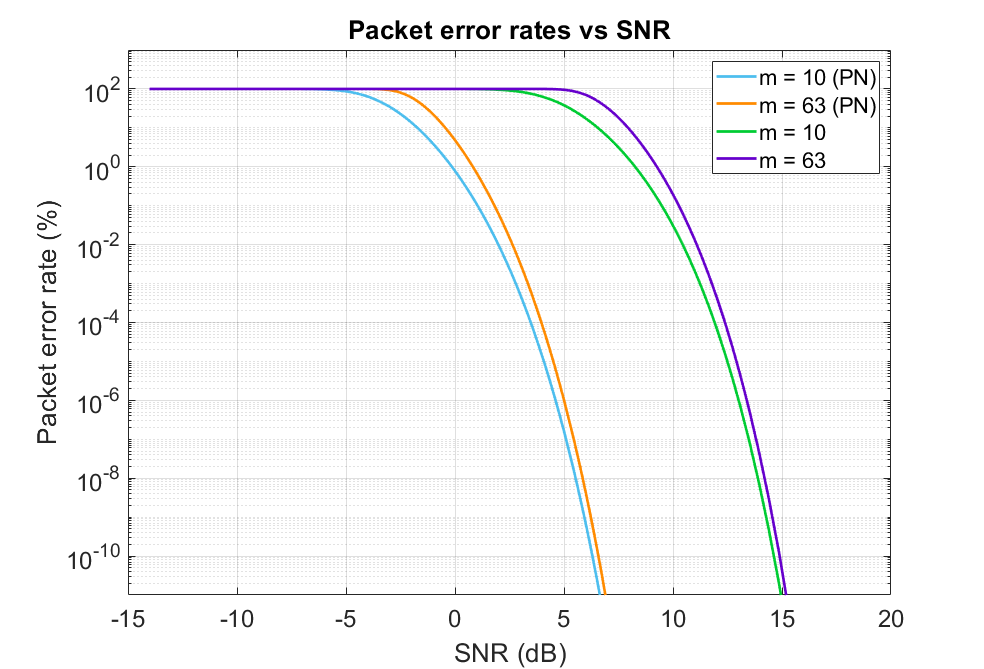
\includegraphics[width=0.99\columnwidth]{snr2.png}
\caption{Plot of PER vs SNR.}
\label{fig:snr}
\end{figure}

\begin{figure}[t!]
\centering
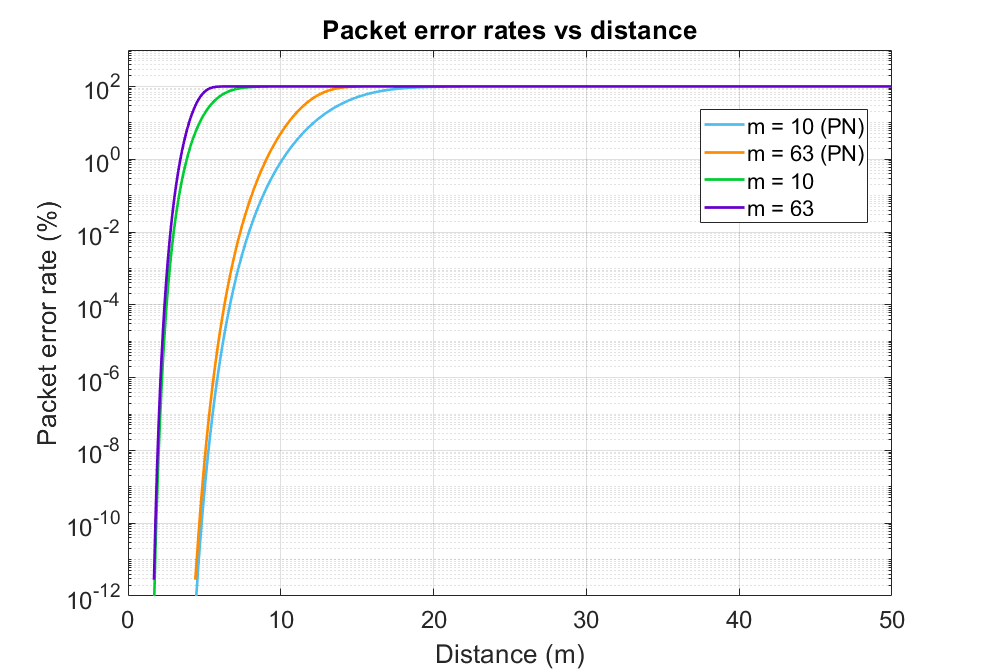
\includegraphics[width=0.99\columnwidth]{distance2.png}
\caption{Plot of PER vs Distance.}
\label{fig:distance}
\end{figure}

\begin{table}[h!]
    \renewcommand{\arraystretch}{1.25}		% Incrementa un poco la altura de las filas
    \centering
    \caption{Constant parameters used for the BER calculation.}	% Los rótulos deben ir arriba de la tabla
    \label{tab:variables}
    \begin{tabular}{l|l}					% {l|l} define la alineación de las columnas y la línea divisoria
    \hline \hline
    \textbf{parameters}        &    \textbf{Value}\\
    \hline
    $D_{t}$          &   1\\
    $D_{r}$          &   1\\
    $P_{t}$          &   7 dB\\
    $P_{noise}$      &   -53 dB\\
    \hline \hline
    \end{tabular}
\end{table}

These values were selected in order to represent a scenario with noisy conditions, real power of mircrocontroller transmission, and directivity of the isotropic antennas used to simplify calculations. Furthermore, the effect of $m$ on the packet error rate can be observed. In larger transmitted packets, a symbol is more likely to be received in error, so the percentage of erroneous packets increases earlier and with a steeper slope. In the previous plots, it is chosen real packet sizes that are used by the system to transmit messages in each micro-interval.

Also, it can be observed that in a transmission that does not use Spread Spectrum with PN sequence, the packet error increases faster and steeper than the IEEE 802.15.4 PHY transmission. This is one of the benefits of the protocol used by the IoT system implemented by the TaIO systems company.


\subsection{Implementation of the scenarios}
\label{sec:implScenarios}


Each feature described in the previous section is composed of different scenarios, which require the implementation of functions, sub-modules, and routines. One of these sub-modules is in charge of the cryptographic process, which allows the testing of the system under different security modes. The operation modes use key establishment protocols, that allow both  points of the system (GVA and Tag) to establish a shared secret talk in an insecure communication channel. It later uses several layers with message authentication codes based on hashes, schemes block encryption, and binary-to-text encoding.

All this message authentication process was implemented in both the simulated Tag and the GVA, allowing the authentication of  association request messages and sensor data messages. These authentication levels define the following different system security modes.

\begin{itemize}
    \item MODE 0: No message authentication.
    \item MODE 1: Authentication of association request messages.
    \item MODE 2: Authentication of association request messages and sensor data messages.
\end{itemize}

Another aspect to take into account when defining the scenarios is the limit of the number of tags that the system can handle in the different security modes. In the case of mode 0, the system is capable of handling up to 50 tags, for mode 1 it is  limited to 10 tags, and for mode 2, the system can manage a maximum of 5 tags.

On the other hand, the feature that contains scenarios where the tags have disconnection periods requires the implementation of a process of blocking messages, from the tag to the server. For this reason, a communication mechanism was developed between the BBD testing script and the NPHKM. This mechanism allows the configuration of a flag that represents the connection status of the tags. The flag is requested by each tag when its tasks are finished (before sending yield), and enables or disables the sending of messages to simulate the disconnection. In the synchronization process, this flag is defined as "SET CONNECTION STATUS". To define the scenarios present in each characteristic, two or more of the following simulation characteristics were combined.

\begin{itemize}
    \item Security mode.
    \item Number of tags.
    \item Number of authenticated tags.
    \item Simulation time.
    \item Disconnection time.
    \item Packet loss percentage.
\end{itemize}

The behavior library offers the ability to label scenarios and set special behaviors for groups of scenarios. Moreover, Behave can execute processes before starting the execution of scenarios (beforeAll) or after it (afterAll), or set configurations and execute functions with the labels (beforeLabel and afterLabel). In this implementation, the beforeAll method was used in order to compile and execute the simulation system. In this way it is ensured the correct operation and execution of the process within a BDD scenario. The beforeTag was also used to establish the percentage of packet loss and the appropriate number of tags.

Figure \ref{fig:bddScenario1} shows the definition of an implemented scenario, in which several simulation characteristics were combined such as number of tags, packet-loss percentage, simulation time, and security mode. An example of the use of labels is shown in the first line of this scenario. Another scenario is shown in Fig. \ref{fig:bddScenario2}, in which the behavior of the system is checked with multiple tags in the event of disconnection periods.

\begin{figure}[t!]
\centering
\begin{lstlisting}[style=scenarioStyle]
&@smode.mt.noise.66&
Scenario: <{3} tags are already to establish communication and send sensor data with packet loss percentage of [5]%>
    
    Given the simulated system is running in security mode "2"
    When the association process is executed for all the tags
    Then I should get sensor data from multiple tags for 1 hours
    And ensure there is no lost data
\end{lstlisting}
\caption{BDD Scenario example with packet loss.}
\label{fig:bddScenario1}
\end{figure}

\begin{figure}[t!]
\centering
\begin{lstlisting}[style=scenarioStyle]
&@special.loggedData.4&
Scenario: <{10} tags are already to establish communication and store data in a disconnetion period%>
    
    Given the simulated system is running in security mode "0"
    When the association process is executed for all the tags
    And the tags disconnet for 2 hours
    And the tags establish connection again
    Then I should get sensor data logged from all the tags
\end{lstlisting}
\caption{BDD Scenario example with disconnection period.}
\label{fig:bddScenario2}
\end{figure}

A total of 98 scenarios were defined, using different combinations of simulation configurations, in order to face the system in multiple situations and ensure the quality of the firmwares present in the components of the IoT environment. The Table \ref{tab:scearios} shows the number of scenarios for each feature and the characteristics that were combined for its implementation.

\begin{table}[h!]
\renewcommand{\arraystretch}{1.25}		% Incrementa un poco la altura de las filas
\centering
\caption{Implemented scenarios for each feature.}	% Los rótulos deben ir arriba de la tabla
\label{tab:scearios}
\begin{tabular}{l|l|l|l|l|l|l|l}					% {l|l} define la alineación de las columnas y la línea divisoria
\hline \hline
\textbf{Iot system working...}     &   \textbf{Qty}     &	\textbf{C1}     &\textbf{C2}    &\textbf{C3}    &\textbf{C4}    &\textbf{C5}    &\textbf{C6}\\
\hline
with a single tag               &   3   	            &	X   &   &   &   &   &   \\
with multiple tags              &   19  	            &	X   & X &   &   &   &   \\
with packet loss                &   54   	            &	X   & X &   & X &   & X \\
with disconnections      &   16   	            &	X   & X &   & X & X &   \\
with unauthorized tags          &   6   	            &	X   & X & X &   &   &   \\
\hline
\multicolumn{8}{l}{Qty: Quantity of scenarios}	\\
\multicolumn{8}{l}{C1: Security mode, C2: N°of tags, C3: N° of authenticated tags,}	\\
\multicolumn{8}{l}{C4: Simulation time, C5: Disconnection time,}	\\
\multicolumn{8}{l}{C6: Packet loss percentage}	\\
\hline \hline
\end{tabular}
\end{table}

The number of scenarios varies in each feature, depending on the number of characteristics that are combined and the impact it has on the operation of the system. For example, the percentage of packet loss has great relevance and impact on the process of associating the tags to the sensor network, so, a large number of scenarios were defined to corroborate that no failure is triggered. Instead, the tests with unauthorized tags did not present a significant impact on the operation of the system. Therefore, the number of defined scenarios is enough to corroborate the robustness of the system to these types of conditions.


\section{Generation of electric current graphs in the simulated tag}
\label{sec:current}


An additional functionality developed for the simulated system is the ability to obtain a graph of the electric current consumption based on the measurement of the time that the tag remains in different operating modes. To capture the consumption measurements in a real tag, the Otii Arc equipment of the QOITECH company was used. It is a power analyzer and supply that allows feeding a load, recording and displaying currents, voltages, and UART registers in real time.

In the case of current measurements, the equipment has a resolution of nA with sampling frequency up to 4 ksps. It has a desktop application that allows us to store measurement information and export the data in popular formats such as csv. The Table \ref{tab:currents} shows the tag's main operating modes and their corresponding current consumption.

\begin{table}[h!]
    \renewcommand{\arraystretch}{1.25}		% Incrementa un poco la altura de las filas
    \centering
    \caption{Current consumption of the main operation modes of the tag.}	% Los rótulos deben ir arriba de la tabla
    \label{tab:currents}
    \begin{tabular}{l|l}					% {l|l} define la alineación de las columnas y la línea divisoria
    \hline \hline
    \textbf{Modes}        &    \textbf{Current (mA)}\\
    \hline
    Sleep               &   0.034\\
    Rx                  &   31.2\\
    Tx                  &   36.1\\
    Sensor Callback     &   23.8\\
    \hline \hline
    \end{tabular}
\end{table}

To generate the simulated tag current graph, markers were placed at the beginning and end of each operation modes. These markers are key messages included in the tag debugging records, which allow determining the duration of each process to later relate them to the corresponding current consumption measured in the real scenarios. The marker structure is simple, it has a message that indicates the operating mode and the running time of the system, as shown in Fig. \ref{fig:markers}.

\begin{figure}[t!]
\centering
\begin{lstlisting}[style=scenarioStyle]
    Current consumption ==> MODE: TX init at 9628843
    Current consumption ==> MODE: TX end at 9628849
\end{lstlisting}
\caption{Example of current consumption markers.}
\label{fig:markers}
\end{figure}

After capturing all the markers in the tag debugging messages, the data was stored generating the time intervals given in each operating mode, to finally generate equidistant time vectors for graph construction, with the data for each step of the system's clock. Each unit of time is assigned to its corresponding current value.


\section{Results}


The results of this work are shown below and they are organized by sections that describe the main advantages of the behavioral testing system.


\subsection{Speed factor}


As mentioned in section \ref{sec:implScenarios}, 98 scenarios were implemented and executed, obtaining measurements of the time simulation and the real time execution. The simulation execution time is the time it takes to scenario to run, and the real execution time refers to how much time has elapsed in the simulated system clock. Fig. \ref{fig:scenarios1} shows the measurements of these times.

\begin{figure}[t!]
\centering
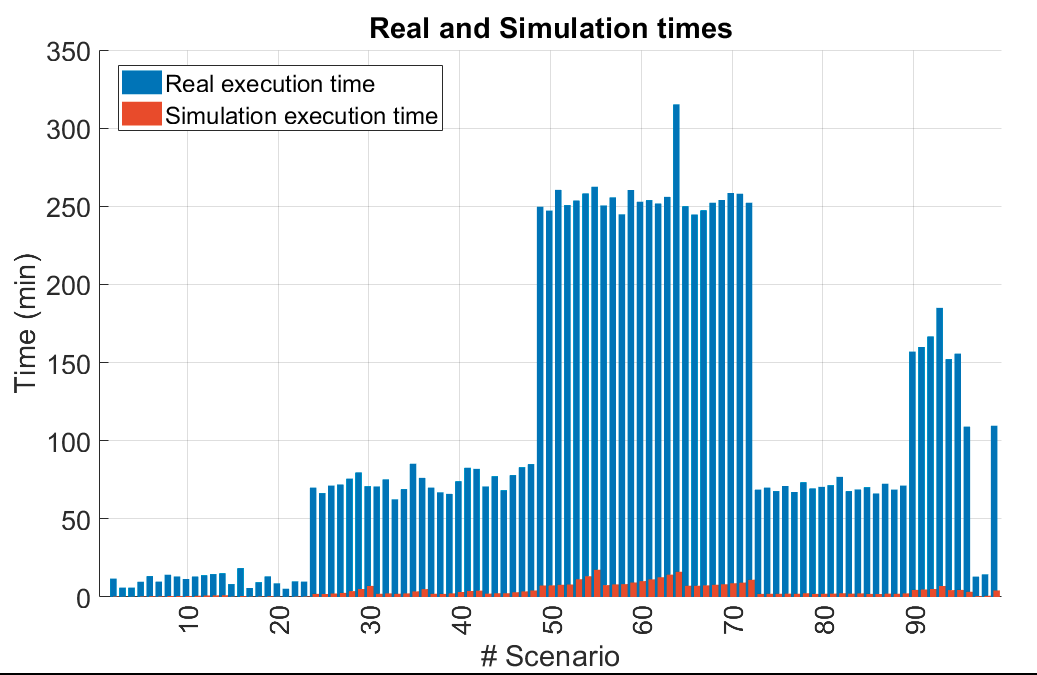
\includegraphics[width=0.95\columnwidth]{scenarios4.png}
\caption{Real and simulation times.}
\label{fig:scenarios1}
\end{figure}

The magnitude difference between the execution and simulation times are significant, and it is observed that the execution durations vary between the different scenarios defined in the behavioral testing tool. This is mainly due to one of the characteristics defined in the implementation of the scenarios: the number of tags. Also, it is intuitive to think that the number of simulated processes has an impact on the machine computational load where they are executed. Fig. \ref{fig:speed} shows the impact of the number of tags on the speed factor of the simulated system.

\begin{figure}[t!]
\centering
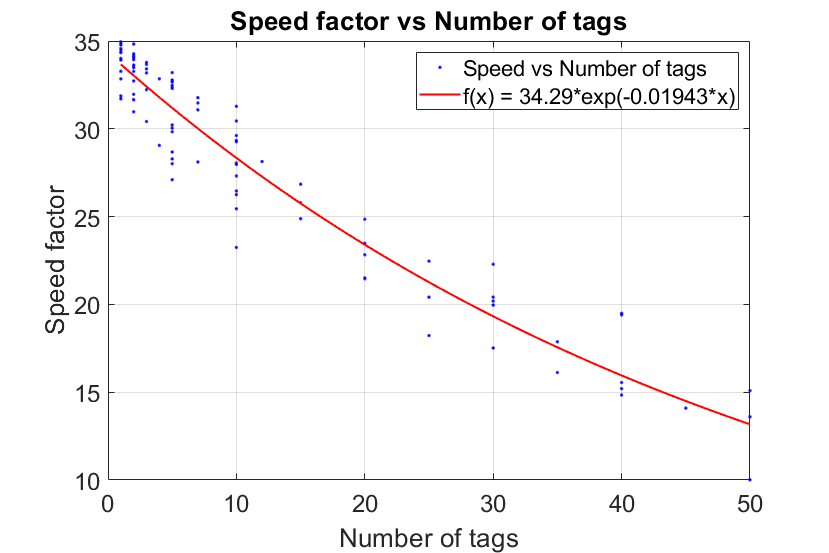
\includegraphics[width=0.95\columnwidth]{speedFactor2.png}
\caption{Speed factor vs. No. Tags.}
\label{fig:speed}
\end{figure}

The Table \ref{tab:speed} shows the average values of the speed factor of the simulated system versus the real system, for different number of tags. In the case of a single tag, the behavioral testing system is capable of executing a 4-hour test in  7.3 minutes, which allows the company's development team to streamline the testing and quality control process in the different system firmwares.

\begin{table}[h!]
    \renewcommand{\arraystretch}{1.25}		% Incrementa un poco la altura de las filas
    \centering
    \caption{Speed factor for different number of tags.}	% Los rótulos deben ir arriba de la tabla
    \label{tab:speed}
    \begin{tabular}{l|l}					% {l|l} define la alineación de las columnas y la línea divisoria
    \hline \hline
    \textbf{No. Tags}        &    \textbf{Speed factor}\\
    \hline
    1       &   33.92\\
    2       &   33.23\\
    5       &   30.76\\
    10      &   27.89\\
    20      &   24.28\\
    30      &   20.71\\
    40      &   16.43\\
    50      &   12.90\\
    \hline \hline
    \end{tabular}
\end{table}

The acceleration factor for the simulated system exhibits a behavior that adjusts to a decreasing exponential curve. This is due to the multiprocessing capacity of the computer, running multiple processes on different cores and threads. The use of system resources against the simulation system implemented is beyond the scope of this study.


\subsection{Debugging of the whole system}


Figure \ref{fig:simulated-system} shows a screenshot of the simulation system, running and showing the debugging messages of the system. According to this figure, both the C-Process and the Gateway are capable of storing debugging messages (logs) of the entire simulation process. The simulated system stores these messages in separate text files, which are updated in real time, allowing a follow-up of each step and task performed by the different components. In addition, the GVA has debugging messages to check the reception and sending of messages to the gateway, authentication of failures even any failure of the GVA itself.

\begin{figure*}[t!]
\centering
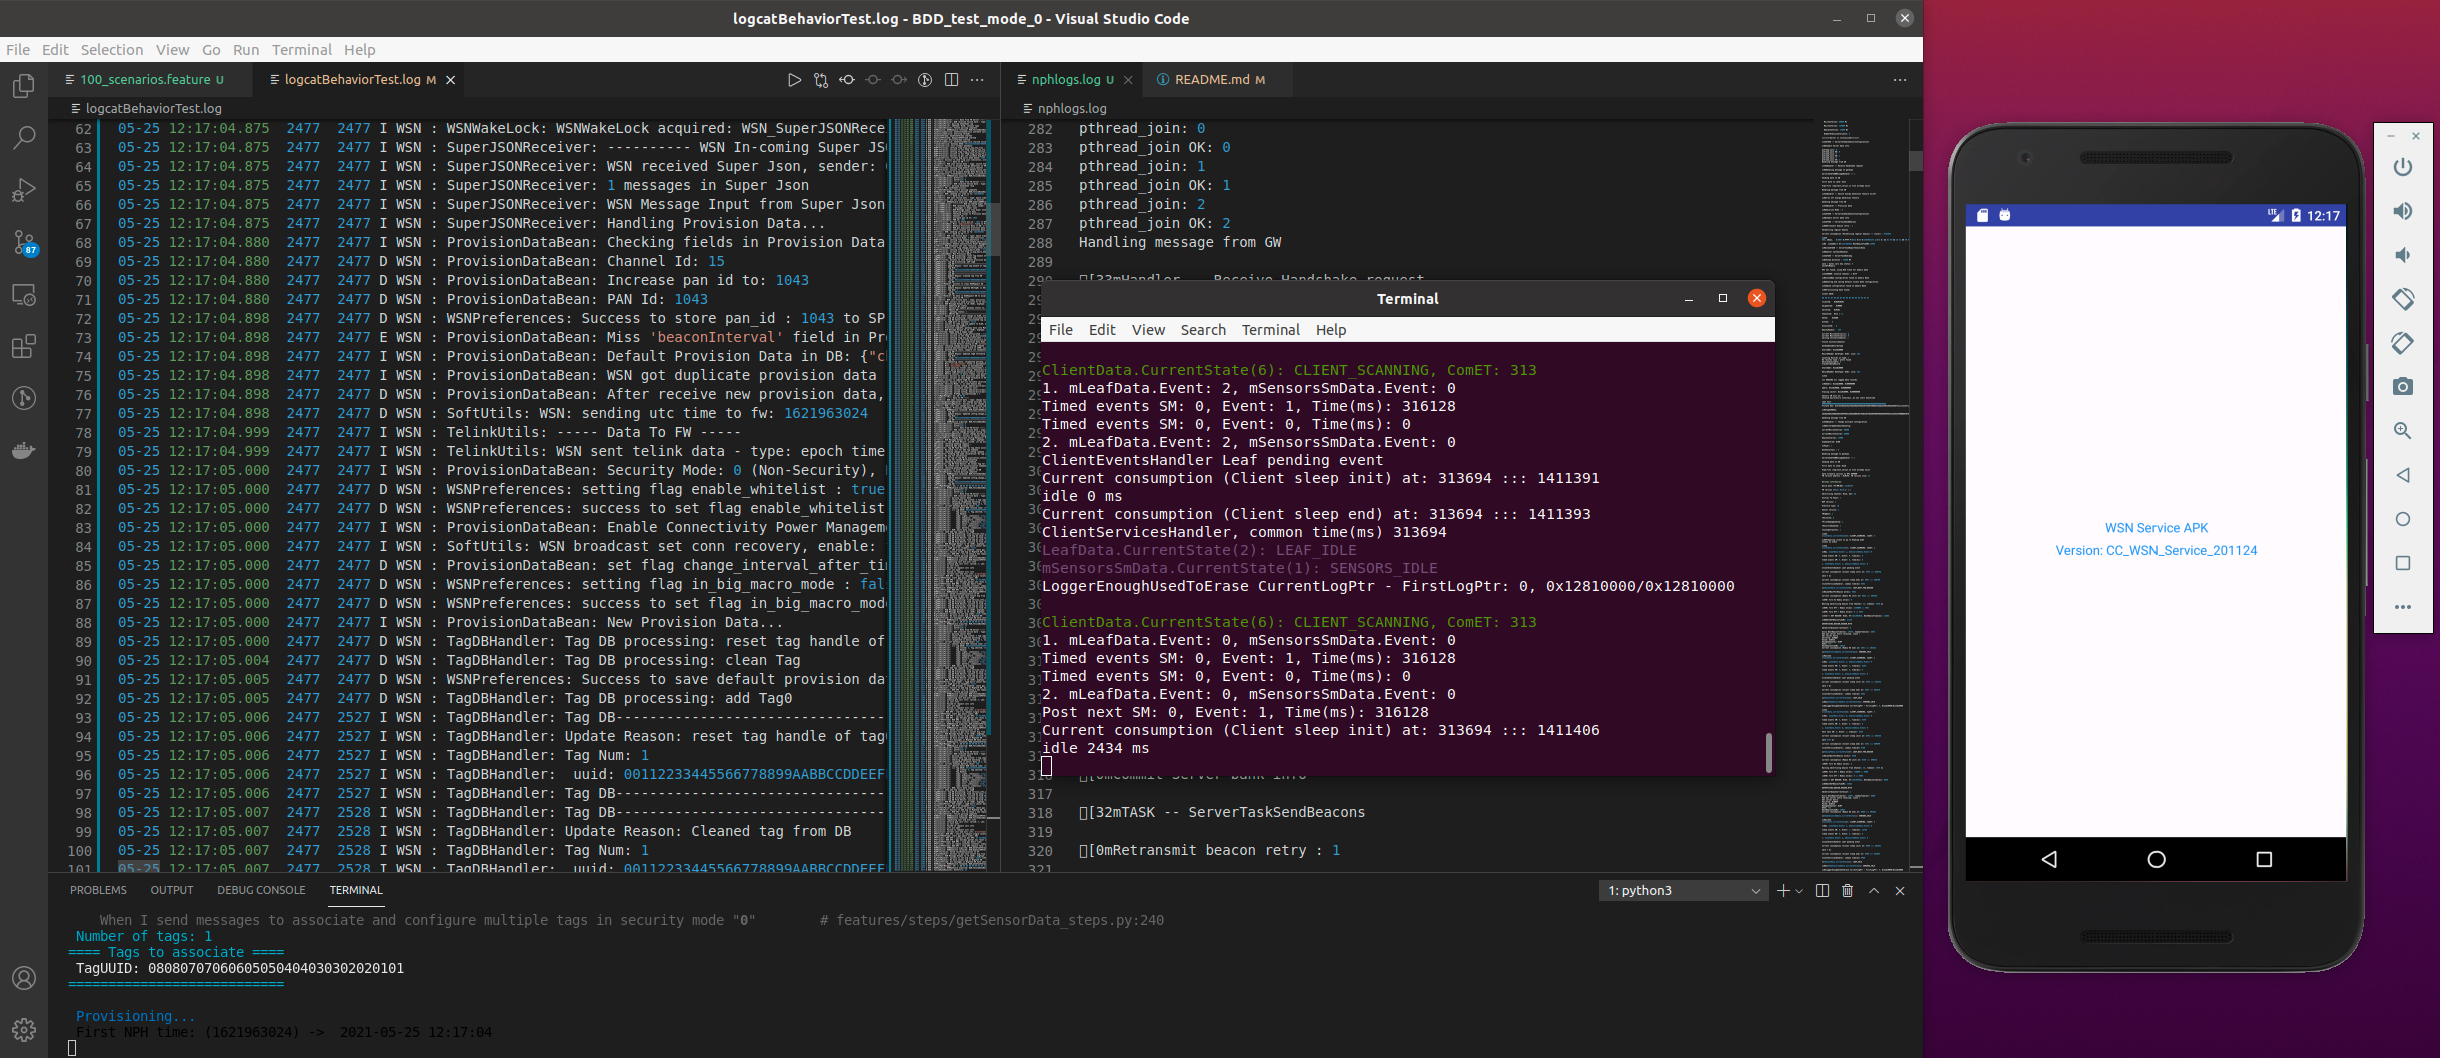
\includegraphics[width=0.99\textwidth]{simulated.png}
\caption{Simulated system running.}
\label{fig:simulated-system}
\end{figure*}

This mechanism corroborates in detail the correct operation of each routine, subroutine, or function executed in any of the components. Therefore, it facilitates the detection and correction of faults that are not detected in macro behaviors, such as those tested in the BDD scenarios.


\subsection{Current consumption graph}


As mentioned in section \ref{sec:current}, a mechanism was developed to generate electric current graphs for the tag. The graphs were compared with those obtained by the power analyzer in a real scenario. Fig. \ref{fig:microIntervals} shows a comparison between the graphs for a fragment of the system simulation process, specifically a group of microIntervals. In addition, Fig. \ref{fig:sendMessage} shows a comparison of the electric current graph for the data sending process in each micro interval.

\begin{figure}[t!]
\centering
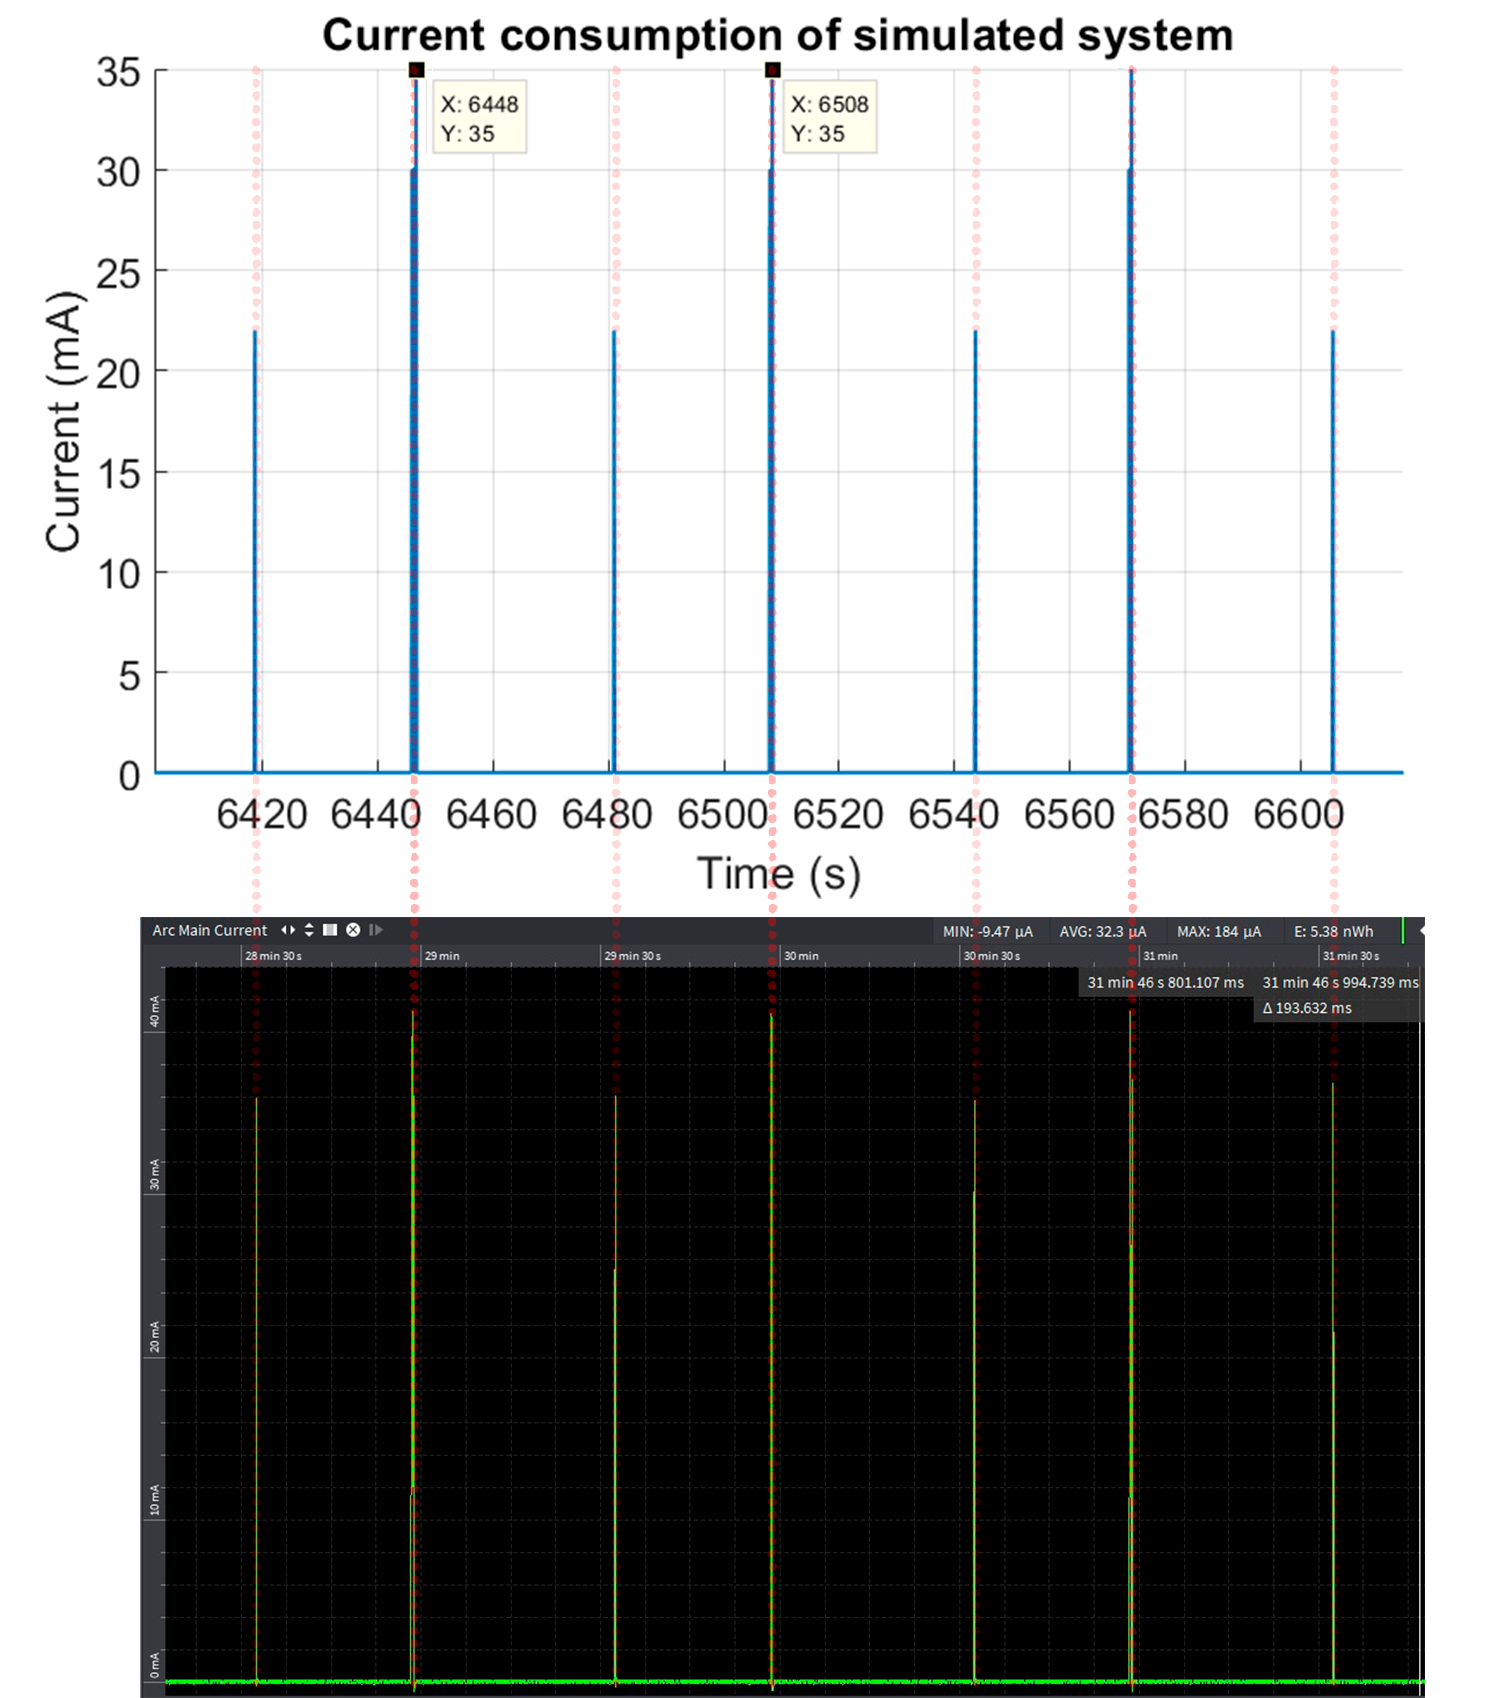
\includegraphics[width=0.99\columnwidth]{microIntervalsAll.png}
\caption{Micro intervals consumption graph.}
\label{fig:microIntervals}
\end{figure}

\begin{figure}[t!]
\centering
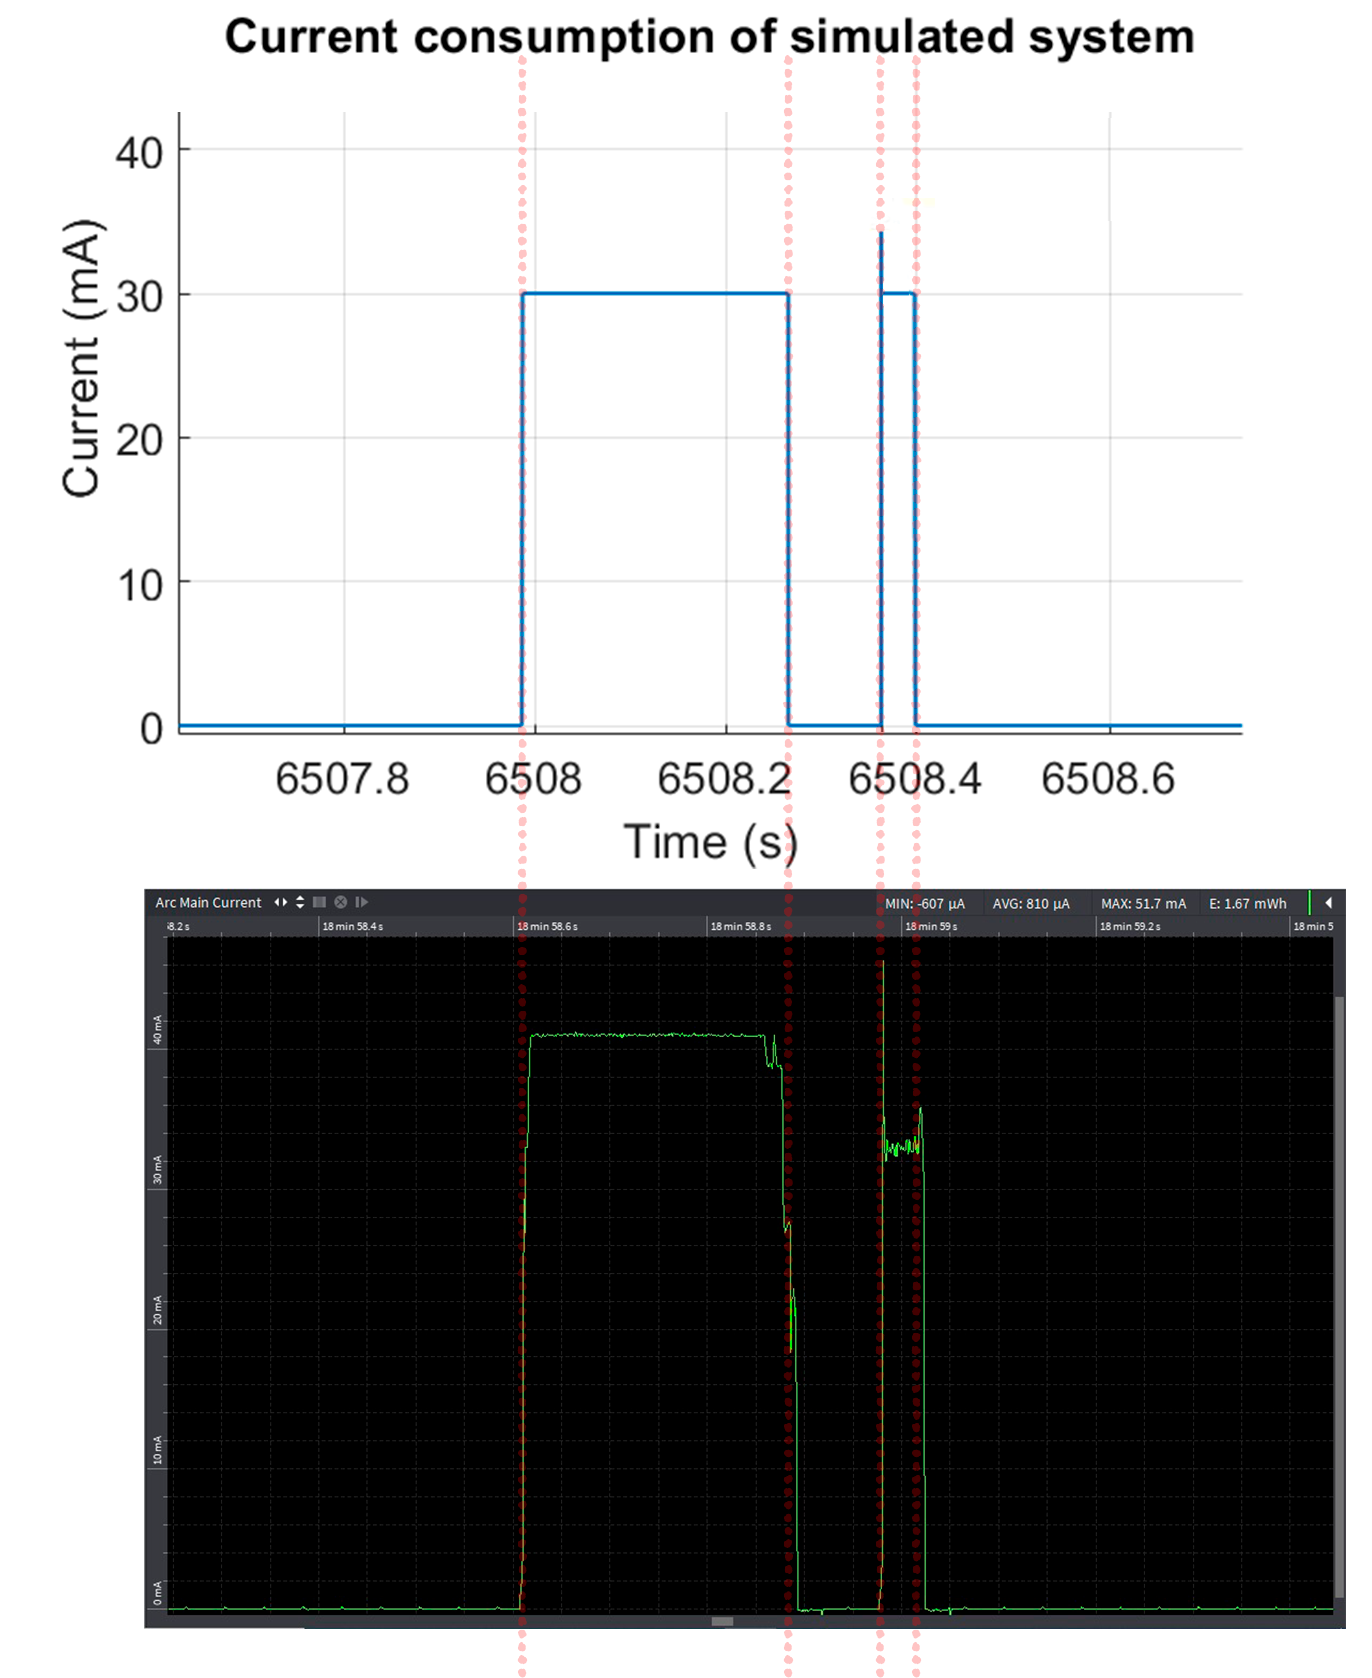
\includegraphics[width=0.99\columnwidth]{microIntervalsOne.png}
\caption{Graph of electric current consumption for sending messages.}
\label{fig:sendMessage}
\end{figure}

At each of the intervals, the tag requests information from the sensors, waiting the arrival of a new reference beacon, to respond with information from the sensors or a live message. The duration between each micro-interval is constant. For this reason, it is observed that the process is periodic with a period of 60 seconds (micro interval).

In the process of sending data in each micro interval, the tag presents two kind of current pulses. The pulses of lower amplitude represent the process of obtaining data from the sensors, and the higher amplitude pulses represents the transmission of the corresponding message for each interval.

The results obtained by the current graph generation mechanism allow us to observe the impact of different processes executed on the tag. In addition, this mechanism could be used to analyze the impact on current consumption, when new functionalities within the tag are implemented (when server search, association, and data sending processes are modified).


\subsection{Bug fixes}


During the process development of the automatic behavioral testing tool, the TaiO System Company provided the support service for the IoT system project, receiving different bug reports in some functionalities. One of these bugs was related to the verification of threshold values for the sensor configurations. These values are used to activate interruptions or alarms in the tag sensors, and thus report anomalous values during their operation. These values are configured from a web platform that verifies the limit values are within a certain range. And finally, it send this information to the GVA, which is in charge of configuring the sensor network with these parameters.

The error due to a failure in the verification of these parameters, which caused a threshold value higher than the established, unleash an erratic behavior in the system. Therefore, the development team had to debug the system in order to replicate the error and later correct it.

A single tag scenario was used and the simulated GVA was configured to send a configuration packet, with the same scenario conditions. After executing this scenario, we proceeded to review the debugging messages obtained from the different components of the simulated system. It shows that there was an inconsistency between the message received by the gateway and the message sent to the server.

As in all agile development methodology based on tests, the first step is to define the test scenario. After the component that caused the error is identified, a new scenario had to be designed to verify that the threshold configuration is transmitted correctly to all the system components. Fig. \ref{fig:bddBug} shows the scenario definition. Then, the scenario was executed to verify that it failed and, finally, a solution was implemented to pass the test.

\begin{figure}[t!]
\centering
\begin{lstlisting}[style=scenarioStyle]
Scenario: <{1} tags are already to establish communication and be configured>
    
    Given the simulated system is running in security mode "0"
    When the association process is executed
    And the configuration is sent by the GVA
    Then the tag should receive the configuration correctly
    And sent the sensor data in the next macro interval
\end{lstlisting}
\caption{BDD Scenario implemented to correct the threshold bug.}
\label{fig:bddBug}
\end{figure}


\subsection{Optimization of the development time}


New development tasks were assigned to the company team in order to strengthen the knowledge and familiarization with the IoT system firmware. These tasks were related to the implementation of new functionalities and modification of some existing ones.

One of these development tasks modifies the sensor message forward process. When a tag sends a sensor information package and it is lost during the process, the server detects the loss and sends a reconnection beacon. Then, the tag stores the lost data in its flash memory, to later put it forward in the next macro frame. When the IoT system operates under conditions of high noise levels, the previous process can be repeated frequently, having to store and read information from flash memory.

The new implementation of the forwarding process aimed to avoid large data storage, and instead try to put forward the message during the same macro frame. In this process, the tag looks for using non-volatile storage only when new information is retrieved from sensors.

To carry out this implementation, the development team used the automatic behavioral testing tool. Particularly, they used scenarios that included packet loss to simulate the conditions this new data transfer process is executed. Once the changes were made into the simulated system, including the possibility of debugging information in all the components and the rapid execution of the scenarios, the task was completed in a shorter time than the expected by the company. Moreover, it allowed to correct errors during the implementation before carrying out tests in a real scenario, thanks to the possibility of testing multiple scenarios with different percentages of packet loss and execution durations.

After the new implementation passed all the BDD tests, it worked correctly in the real scenario, without the need of further changes. The execution time of the scenario simulation was 1 hour and 29 minutes, which means 50 hours of real execution time. Table \ref{tab:scenariosNewImpl} shows the executed scenarios time information.

\begin{table}[h!]
    \renewcommand{\arraystretch}{1.25}		% Incrementa un poco la altura de las filas
    \centering
    \caption{Times of the scenarios used for the new implementation.}	% Los rótulos deben ir arriba de la tabla
    \label{tab:scenariosNewImpl}
    \begin{tabular}{l|l|l|l}					% {l|l} define la alineación de las columnas y la línea divisoria
    \hline \hline
    \textbf{Scenario}        &    \textbf{Repetitions} &    \textbf{Total simulation time} &    \textbf{Total real time}\\
    \hline
    1 hour of DC      &   20   &   0.5898 &   20 hours\\
    2 hour of DC      &    5   &   0.2949 &   10 hours\\
    4 hour of DC      &    5   &   0.5896 &   20 hours\\
    \hline
    \multicolumn{4}{l}{DC: Data collection}	\\
    \hline \hline
    \end{tabular}
\end{table}

In the middle of the execution of these scenarios, changes were made in the code to correct errors into the implemented solution. Those as the debugging, compilation, and flashing processes in the real scenario are more complex and unexpected, and can increase the development time. Table \ref{tab:advantageNewImpl} shows the old and the new implementation storage times,  assuming 2 minutes for macro interval, packet loss of 20 percent, and the flash memory size of 389,120 bytes. In here, the new implementation shows a great performance over the old one, specifically in increasing the capacity to store information in flash memory for more days of execution.

\begin{table}[h!]
    \renewcommand{\arraystretch}{1.25}		% Incrementa un poco la altura de las filas
    \centering
    \caption{Storage times of the old and new implementations.}	% Los rótulos deben ir arriba de la tabla
    \label{tab:advantageNewImpl}
    \begin{tabular}{l|l}					% {l|l} define la alineación de las columnas y la línea divisoria
    \hline \hline
    \textbf{Implementation}        &    \textbf{Max days to store}\\
    \hline
    Old      &   57  \\
    New      &   287  \\
    \hline \hline
    \end{tabular}
\end{table}

The new implementation reduces the number of logged messages in 5 times. Therefore, it is capable of store data in flash memory through more days. Moreover, if the macro interval is greater, the probability of logging data is reduced and the number of days stored in memory increases.


\section{Conclusions}


In this work, the design and implementation of an automatic behavioral testing system, for an IoT environment for the TaIO Systems Company was carried out. It is capable to detect and correct errors, verify compliance with system requirements, and optimize the development process.

A simulation system was implemented to execute, synchronize, and communicate all the systems components. In this simulation, it is possible to implement different test scenarios based on the BDD development strategy, which allows the system to face different simulation conditions present in the normal operation of real systems.

The behavioral testing system reach simulations of real scenarios with a speed factor greater than the real system. The system presents a reduction in the speed factor when the number of simulated tags is increased. Also, it is possible to retrieve debugging messages from the entire system and to decrease the time that is required for detection and correction of errors, as well as the implementation time of new functionalities.

The implementation of electric current plots for the tag is very close to the real behavior of this variable. This feature can contribute to the impact analysis of implementation changes into the firmware and the addition of new functionalities related to the system's current consumption.


\section{Future work}


A new multi-process simulation strategy could be implemented to improve the performance of the simulation system in the presence of a large number of tags. This strategy should require a restructuring work of the simulation system and the use of new tools and computational resources such as GPUs.

To carry out simulated electric current measurements that allow statistical data analysis, for example current average in a long-duration process, it might require a modification of the simulation and synchronization system for multiple processes, as well as the data acquisition of tag's electrical current consumption in large tasks and subroutines sets.


% Use section* para los agradecimientos (evita que se numere como una sección adicional).
\section*{Acknowledgment}


This work is the result of an advanced and practical experience developed at TaIO System Company. Authors would like to thank Universidad de Nariño and TaIO Systems Company for the academic and financial support.


% Sección de referencias
\bibliographystyle{IEEEtran}		% Ajusta el formato de las referencias
\bibliography{referencias}			% Nombre del archivo que contiene las referencias


\end{document}


